\documentclass[11pt,letterpaper]{article}
\usepackage{cogsys}
%\usepackage{cogsysapa} % deprecated!
\usepackage[T1]{fontenc}
\usepackage{times}
\usepackage[pdftex]{graphicx} % use this when importing PDF files
\usepackage{booktabs}
\usepackage{amsmath}
\usepackage{algorithm}
\usepackage{algpseudocode}

% natbib required to produce author-year citations;
% apacite is not properly supported and may lead to errors
\usepackage{natbib}
\setlength{\bibsep}{0.75ex}


\newcounter{rpostulate}
\newcounter{opostulate}
\newcounter{ppostulate}
\newcounter{lpostulate}

\newenvironment{rpost}{%
  \stepcounter{rpostulate}%
  \par\noindent
  \hangindent=2.5em\hangafter=1%   % wraps postulate text to after "R1."
  \textbf{R\therpostulate.}~\ignorespaces
  \setlength{\parindent}{0pt}%     % follow-up paragraphs align with "R"
  \setlength{\parskip}{4pt}%
}{%
  \par\medskip
}

\newenvironment{opost}{%
  \stepcounter{opostulate}%
  \par\noindent
  \hangindent=2.5em\hangafter=1%   % wraps postulate text to after "O1."
  \textbf{O\theopostulate.}~\ignorespaces
  \setlength{\parindent}{0pt}%     % follow-up paragraphs align with "O"
  \setlength{\parskip}{4pt}%
}{%
  \par\medskip
}

\newenvironment{ppost}{%
  \stepcounter{ppostulate}%
  \par\noindent
  \hangindent=2.5em\hangafter=1%
  \textbf{P\theppostulate.}~\ignorespaces
  \setlength{\parindent}{0pt}%
  \setlength{\parskip}{4pt}%
}{%
  \par\medskip
}

\newenvironment{lpost}{%
  \stepcounter{lpostulate}%
  \par\noindent
  \hangindent=2.5em\hangafter=1%
  \textbf{L\thelpostulate.}~\ignorespaces
  \setlength{\parindent}{0pt}%
  \setlength{\parskip}{4pt}%
}{%
  \par\medskip
}

 % First page headings for accepted submissions.
\cogsysheading{X}{20XX}{1-6}{X/20XX}{X/20XX}
 % First page headings for poster submissions.
%\cogsysposterheading{First}{2012}{1-18}

\ShortHeadings{Grammar Induction Through Compositional Chunking}
              {K.\ Singaravadivelan and P.\ Langley}

\begin{document}

\title{\textsc{Trellis}: Grammar Induction Through Compositional Chunking}

\author{Karthik Singaravadivelan}{ksingara3@gatech.edu}
\author{Pat Langley}{something goes here}
\address{Institute for the Study of Learning and Expertise,
         2164 Staunton Court, Palo Alto, CA 94306 USA}
\vskip 0.2in

\begin{abstract}
Humans routinely recover hierarchical structure from sequential experience: a stream of words is parsed into phrases, a sequence of moves is grouped into a familiar opening, a row of pixels is read off as a written word. Two longstanding cognitive traditions have addressed pieces of this ability separately. Concept-formation systems organize observed instances into taxonomic hierarchies that support recognition and prediction, but they treat instances as flat attribute--value vectors with no internal structure. Chunking systems compose recurring patterns into hierarchical wholes, but they typically lack any account of the categorical generalization that lets a chunk recognize instances it has never literally seen. In this paper, we present a theory that unifies the two by treating every element of an experience as having both a \emph{content} description, which names its parts, and a \emph{context} description, which names its surroundings, and by organizing the two descriptions across two parallel taxonomic hierarchies. We instantiate the theory in \textsc{Trellis}, an implemented system that uses two Cobweb hierarchies as its taxonomic substrate, incrementally parses experiences into partonomic structures, and inverts the same machinery to generate from memory. We evaluate \textsc{Trellis} on three synthetic context-free grammars of increasing complexity and report parse F1 between 86\% and 99\% with 100\% from-scratch generation grammaticality across all grammar sizes.
\end{abstract}

\section{Introduction}

The cognitive systems literature has long sought computational accounts of how humans recover hierarchical structure from sequential experience. Two of its most enduring traditions --- concept formation and chunking --- have each captured something real about this ability, but each has historically lacked what the other supplies. Concept formation has produced incremental, unsupervised systems that organize instances into taxonomic hierarchies and support generalized recognition, but its representational vocabulary treats every instance as a flat attribute--value vector with no internal structure. Chunking has produced models in which long-term memory aggregates recurring configurations into hierarchical wholes, but those models typically match input exactly and do not generalize across structurally similar instances. Neither tradition, on its own, gives a complete account of the phenomena.

In this paper we propose a theory that unifies the two by making every element of an experience carry both a \emph{content} description, which names its parts, and a \emph{context} description, which names its surroundings. The theory assumes the existence of taxonomic hierarchies of the kind that Cobweb \citep{fisher-cobweb} produces, and adds a small set of postulates that together support the incremental parsing of an experience into chunks and the inverse generation of an experience from memory. We instantiate the theory in \textsc{Trellis}, an implemented system that uses two Cobweb hierarchies --- one organizing the content descriptions, one organizing the context descriptions --- as the substrate over which parsing, generation, and learning all run. We evaluate the system on three synthetic context-free grammars and find that it parses with high accuracy, generates 100\% grammatical sentences from memory, and exhibits the kind of incremental, unsupervised learning behavior the postulates predict.

The remainder of the paper proceeds as follows. Section~2 lays out the motivation for combining the two traditions and identifies the natural gap left by all current systems --- the gap our theory aims to fill. Section~3 reviews Cobweb's commitments as a set of postulates and then states our own theory's postulates in the same format, making the points of inheritance and extension explicit. Section~4 describes \textsc{Trellis}, the system we have implemented, and ties each of its components to a specific postulate. Section~5 reports an empirical evaluation against synthetic CFG corpora. Section~6 situates the work alongside other systems that attempt to fill the same gap. Section~7 concludes with a discussion of limitations and avenues for future work. Appendix~A gives the grammars used in evaluation and Appendix~B gives the exact formulas used by the implementation.

\section{Background and Motivation}

One of the most distinctive features of human cognition is its capacity to organize a stream of low-level observations into a layered set of higher-level structures. A reader does not perceive a sentence as a flat list of letters but as a hierarchical arrangement of words, phrases, and clauses; a chess master does not perceive a board as an arrangement of pieces but as a configuration of familiar groupings \citep{chase-simon}; a listener does not perceive a melody as a sequence of notes but as a progression through familiar motifs and themes. This hierarchical organization is not given by the input. It must be inferred, and, in the standard cognitive systems tradition, it must be inferred by the same machinery that learned the lower-level structures in the first place \citep{book-newell-simon, langley-cog-systems}. In the remainder of this section we review the two main computational traditions that have addressed this ability, identify the structural gap that each leaves, and argue that filling the gap requires a unification that the literature has long pointed toward but has rarely committed to in implementation.

\subsection{Concepts and the Concept-Formation Tradition}

The first tradition we will discuss, descended from work on concept formation, treats long-term memory as a taxonomic hierarchy of probabilistic concepts that summarize observed instances \citep{fisher-cobweb, gennari-cobweb-incremental, langley-machine-learning}. Concepts in this tradition are categorical: they generalize across instances, support recognition and prediction, and adapt incrementally as new data arrive. The notion of a concept in psychology has been studied for decades \citep{rips-smith-medin, langley-machine-learning}, with most computational treatments emphasizing recognition over recall and graded membership over all-or-nothing matching. Empirical work on basic-level categories \citep{rosch-basic-level} has identified a privileged level of abstraction at which human classification is fastest and most natural, and the concept-formation literature has long treated this basic-level effect as a constraint on viable hierarchical organizations.

Cobweb \citep{fisher-cobweb} is the most influential system in this line of work. Cobweb maintains a taxonomic hierarchy in which each node is a probabilistic concept summarizing the instances sorted to it, and processes each new instance by sorting it down the hierarchy from the root toward a leaf, at each step considering four restructuring actions (add, create, merge, split) and choosing the one that best improves an evaluation criterion. The system is incremental, unsupervised, and produces hierarchies whose nonterminal nodes correspond to natural levels of generalization within the data. The framework has been extended along many dimensions over the past four decades --- to handle continuous attributes and information-theoretic objectives \citep{cobweb-3-mclelland}, relational structure \citep{trestle-maclellan}, hidden attributes and refined basic-level computation \citep{cobweb-4l-maclellan}, image-classification through a convolutional variant \citep{convolutional-cobweb}, and script-like iterative memory \citep{matsakis-cobweb} --- and it remains the workhorse of incremental, unsupervised category learning in the cognitive systems community.

What every Cobweb variant shares, however, is its representational substrate: an attribute--value vocabulary that admits no compositional structure. An instance is a set of attribute--value pairs. A concept is a probabilistic summary of such sets. Nothing in this vocabulary lets an instance be \emph{composed} of other instances, and nothing in Cobweb's performance vocabulary lets the system parse a sequence of observations into a hierarchical structure. The categorical aspect of cognition is well-served by Cobweb and its descendants, but their representations are fundamentally flat. The hierarchical structure that pervades language, music, chess, action sequences, and scene perception sits outside what Cobweb can express.

\subsection{Chunks and the Chunking Tradition}

The second tradition, descended from work on chunking, treats long-term memory as a partonomic store of recurring configurations \citep{miller-magical-seven, simon-chunking, chase-simon}. The notion of a chunk traces to \citet{miller-magical-seven}, who observed that human short-term memory capacity is approximately constant when measured in chunks rather than in individual items, and concluded that practiced perceivers must aggregate input into larger units that fit within a fixed memory budget. The classic demonstration of this aggregation in expert behavior is \citet{chase-simon}'s study of chess perception, in which masters recalled briefly-presented board configurations far better than novices for meaningful positions but no better for random ones --- evidence that the masters were perceiving boards in chunks rather than in pieces. Together these findings established that long-term memory in skilled performers stores recurring relational configurations and that performance depends on rapid recognition of those configurations from sensory input.

The chunking idea was subsequently formalized in EPAM \citep{epam-richman} and in its successor CHREST \citep{chrest-gobet-lane}, both of which model long-term memory as a discrimination network whose nodes are chunks acquired through repeated exposure. A parallel line of work on chunks as the basic mechanism of procedural learning culminated in Soar \citep{paper-laird-etal}, which uses chunking as a general account of how subgoal solutions are compiled into reusable productions. Each of these systems captures something real about how humans aggregate experience into structured wholes, and each can construct a compositional account of an unfamiliar input from previously-acquired chunks. The relevance of these psychological constructs to natural language has long been recognized: \citet{levinson-paper} argued that the organization of conversational structure is essentially chunk-like, with familiar configurations of utterance types serving as the building blocks of fluent discourse, and earlier computational work on scripts and frames \citep{schank-abelson} treated language understanding as a process of pattern composition rather than rule-driven derivation.

What every chunking system shares, however, is its lack of categorical generalization. A chunk in EPAM either matches an input exactly or fails to match; a production rule in Soar applies to a precisely-shaped situation or it does not. The chunking tradition can compose, but it does not generalize across structurally similar instances. The compositional aspect of cognition is well-served by these systems, but their treatment of category structure is impoverished. A chunk that encodes a particular noun phrase cannot, by virtue of its own machinery, recognize a structurally identical noun phrase whose component words it has never seen.

\subsection{The Gap and Our Proposal}

The two traditions thus have complementary limitations, and the limitations are exactly the strengths of the other tradition. Categorical concepts generalize but do not compose; compositional chunks compose but do not generalize. A theory that treats language, or any other domain whose phenomena exhibit both characters, must combine the two. \citet{langley-concepts-chunks} has recently argued that the two traditions have stayed disjoint for institutional rather than principled reasons, and that a unified theory of mental structures should treat concept-hood and chunk-hood as two aspects of every cognitive representation rather than as two separate kinds of representation. Distributional language representations like Word2Vec \citep{word2vec}, GloVe \citep{glove}, and BERT \citep{bert} have demonstrated, from a very different starting point, that the local context in which a token appears can drive surprisingly rich syntactic categorization; probes can recover part-of-speech tags and constituency structure from intermediate BERT layers with high fidelity \citep{tenney-probing}. These models extract a context-driven categorical structure but do so in a continuous representation that resists explicit compositional analysis. None of the systems we have surveyed combines the categorical generalization of concept formation with the compositional structure of chunking inside a single discrete framework. The natural gap left by this literature is the one our theory aims to fill.

Our proposal does so by taking taxonomic hierarchies of the kind Cobweb produces as a primitive substrate for the categorical aspect of memory, and adding a small set of postulates that govern how the compositional aspect is built up over that substrate. The central claim of the theory is that a chunking system needs not one but two such hierarchies, operating in concert: one that organizes elements by what they are composed of, and another that organizes them by what surrounds them. Together these two hierarchies support the parsing of an experience into chunks, the generation of an experience from chunks, and the incremental absorption of parsed elaborations back into memory. The next section states this theory as a set of postulates in the format established by the concept-formation literature, alongside a parallel restatement of Cobweb's own postulates that the theory inherits.

\section{A Unified Theory of Chunking}

This section presents our theory of chunking as a set of postulates about representation, organization, performance, and learning. Because the theory builds directly on Cobweb \citep{fisher-cobweb}, we first restate Cobweb's own commitments in the same postulate format, in order to make explicit which commitments we inherit and which ones we extend. We then state our own commitments and discuss the central content--context distinction that anchors them.

\subsection{A Review of Cobweb}

Cobweb is an incremental concept-formation system that organizes attribute--value instances into a probabilistic taxonomic hierarchy. The postulates below state Cobweb's commitments about the forms knowledge takes, the arrangement of concepts in long-term memory, the process by which the system handles a new instance, and the way the hierarchy is updated as instances are incorporated.

\subsubsection{Representation Postulates}

We begin by specifying the forms in which knowledge is stored. The following postulates fix these forms.

\begin{rpost}
Knowledge takes two forms: instances and concepts.
\end{rpost}

\begin{rpost}
An instance is a set of attribute--value pairs describing a single observation.
\end{rpost}

\begin{rpost}
A concept is a probabilistic summary of a set of instances, expressed as counts over attribute--value pairs.
\end{rpost}

\begin{rpost}
Cobweb treats the attribute--value pairs within an instance as conditionally independent given a concept, so that each attribute's count distribution at a concept can be considered in isolation.
\end{rpost}

\begin{rpost}
Each attribute's value distribution at a concept is smoothed by a uniform prior, so that unobserved values still receive a non-zero base-rate probability.
\end{rpost}

\subsubsection{Organization Postulates}

Having stated the forms knowledge takes, we now describe the way concepts are arranged in long-term memory.

\begin{opost}
Concepts are organized in a taxonomic hierarchy rooted at a single concept that summarizes all observed instances.
\end{opost}

\begin{opost}
Each non-terminal node in the taxonomy has two or more children that partition the instances it summarizes.
\end{opost}

\begin{opost}
Instances reside as terminal nodes of the taxonomic hierarchy.
\end{opost}

\subsubsection{Performance Postulates}

With these representational and organizational commitments in place, we can describe how Cobweb uses its hierarchy to process a new instance.

\begin{ppost}
An instance is processed by sorting it down the hierarchy from the root toward a terminal node.
\end{ppost}

\begin{ppost}
At each non-terminal node, the instance is routed to the child concept that best fits it under a sorting criterion.
\end{ppost}

\begin{ppost}
Predictions about unobserved attributes of an instance are read from the concept to which that instance is sorted.
\end{ppost}

\subsubsection{Learning Postulates}

Finally, we describe the mechanism by which Cobweb updates its hierarchy as new instances are incorporated.

\begin{lpost}
Learning is incremental, piecemeal, and unsupervised, and it is interleaved with performance.
\end{lpost}

\begin{lpost}
At each non-terminal concept along the sorting path, one of four restructuring actions occurs: add the instance to an existing child, create a new child for the instance, merge two children, or split a child.
\end{lpost}

\begin{lpost}
The action selected at each step is the one that best improves the evaluation criterion at that node.
\end{lpost}

\begin{lpost}
Once sorting terminates, the incorporated instance is installed as a new leaf concept along the path it traversed.
\end{lpost}

\subsection{Postulates for Chunking}

\setcounter{rpostulate}{0}
\setcounter{opostulate}{0}
\setcounter{ppostulate}{0}
\setcounter{lpostulate}{0}

We now state the postulates of our own theory. The theory builds on a longstanding observation that mental structures exhibit both a categorical character, in which they generalize over instances, and a compositional character, in which they decompose into parts. We take taxonomic hierarchies of the kind reviewed in the previous subsection as a primitive substrate for the categorical aspect, and we add postulates that govern how the compositional aspect is built up over that substrate. The theory's central claim is that a chunking system requires two such hierarchies, operating in concert, to support both aspects together: one that organizes elements by what they are composed of, and another that organizes them by what surrounds them. Together these hierarchies support the parsing of an experience into chunks, the generation of an experience from chunks, and the incremental absorption of parsed elaborations back into memory.

\subsubsection{Representation Postulates}

Our theory begins with a position on the forms in which knowledge is stored. As in Cobweb (Section~3.1, R1--R3), knowledge takes the form of instances and concepts; the postulates below extend that representational vocabulary to distinguish primitive from composite elements and to introduce the content--context structure that every element carries.

At the heart of the theory is the notion of an \emph{element}: a unit of structure in the data that may be either a primitive, with no internal composition, or a composite, built from other elements. The theory makes two claims about how an element is represented. First, every element is characterized by what it is made of --- the parts that compose it, when it is composite, or nothing at all, when it is primitive --- which we call its \emph{content}. Second, every element is characterized by what surrounds it --- the discrete relations it bears to its neighbors in an experience --- which we call its \emph{context}. These two characterizations are kept strictly distinct from one another, since each plays a different role in the organization, performance, and learning commitments that follow: the content of an element determines how it participates in chunks, while the context of an element determines where it appears in experiences.

\begin{rpost}
Every element has a content description, which names the parts that compose it.
\end{rpost}

\begin{rpost}
Every element has a context description, which names the discrete relations it bears to surrounding elements.
\end{rpost}

\begin{rpost}
Every element is either a primitive or a composite.
\end{rpost}

\begin{rpost}
A chunk is a composite concept whose instances are themselves built from other primitive or composite elements.
\end{rpost}

\subsubsection{Organization Postulates}

Our representational commitments imply a particular organization of long-term memory, in which the partonomic structure of chunks is supported by a pair of taxonomic hierarchies that play complementary roles.

\begin{opost}
Primitives and composites are jointly organized in a partonomic hierarchy.
\end{opost}

\begin{opost}
An experience is a collection of instances and the relationships between them, represented as a set of primitive elements together with a set of discrete relations among those elements.
\end{opost}

\begin{opost}
The system maintains long-term memory in the form of two distinct taxonomic hierarchies --- a \emph{content hierarchy} organizing the content descriptions of R1, and a \emph{context hierarchy} organizing the context descriptions of R2.
\end{opost}

\subsubsection{Performance Postulates}

With the representational and organizational commitments fixed, we can describe the two processes by which the system uses its memory: parsing, which incrementally builds chunks from a given experience, and generation, which incrementally unpacks chunks back into the elements that compose them.

\paragraph{Parsing.}

\begin{ppost}
Parsing is an incremental process of elaborations on an input experience.
\end{ppost}

\begin{ppost}
A single elaboration generates a set of candidate chunks consistent with the current partial parse.
\end{ppost}

\begin{ppost}
Each candidate chunk is scored against the content and context hierarchies and gated by a recognition threshold.
\end{ppost}

\begin{ppost}
The best-scoring candidate that passes the recognition threshold is committed to the partonomic parse tree as a new composite element.
\end{ppost}

\begin{ppost}
Parsing terminates when no remaining candidate passes the recognition threshold.
\end{ppost}

\paragraph{Generation.}

\begin{ppost}
Generation is an incremental process of expansions on a composite seed.
\end{ppost}

\begin{ppost}
A single expansion produces a candidate leaf consistent with the basic-level concept above the seed's content reference.
\end{ppost}

\begin{ppost}
The candidate leaf is sampled from the content hierarchy and conditioned on the context hierarchy.
\end{ppost}

\begin{ppost}
The sampled leaf is committed to the partonomic generation tree as the seed's expansion, and its content children (if any) become new seeds.
\end{ppost}

\begin{ppost}
Generation terminates when every expanded element is a primitive.
\end{ppost}

\subsubsection{Learning Postulates}

Finally, we describe the mechanism by which the elaborations produced during parsing are absorbed into the two taxonomic hierarchies.

\begin{lpost}
Learning consists of incorporating the elaborations produced by parsing into the two taxonomic hierarchies.
\end{lpost}

\begin{lpost}
Each composite committed during parsing is added to both hierarchies --- its content instance to the content hierarchy and its context instance to the context hierarchy --- while primitives, which carry no content instance, are added to the context hierarchy alone.
\end{lpost}

\begin{lpost}
Each addition follows the standard sorting-with-learning procedure of the taxonomic hierarchy that receives it.
\end{lpost}

\section{The \textsc{Trellis} Chunking System}

We have implemented a system, \textsc{Trellis}, that instantiates the theory of chunking presented in the previous section, built atop the Cobweb framework of Section~3.1. Theories are abstract and require additional assumptions to make them operational. In this section we describe \textsc{Trellis}'s representation, the organization of its long-term memory, its parsing and generation processes, and the way it absorbs the results back into memory. We refer to the earlier postulates wherever a choice can be traced to a theoretical commitment, and to Appendix~B for the exact formulas used by the implementation.

\subsection{Representation}

The \textsc{Trellis} architecture realizes the representational commitments of Section~3.2. To make those postulates concrete, the system adopts a specific encoding for primitives, composites, and the chunks that result from parsing them. The notation resembles attribute--value representations used elsewhere in the concept-formation literature, but elements are constructed and consumed in a distinct way.

Every element in \textsc{Trellis} carries two attribute--value descriptions: a \emph{content instance} and a \emph{context instance}. The content instance names the parts that compose the element; the context instance names the neighbors that surround it. The two are kept separate, and each is routed to its own hierarchy in long-term memory.

Primitives are atomic and have nothing to enumerate, so they carry only a context instance. Composites carry both, as required by R3 and R4.

A composite's content instance contains two attributes naming its left and right children. These attributes store identifiers that point into the context hierarchy, where each child has already been classified. A composite therefore always describes its parts in the same vocabulary as the rest of the system's elements. Figure~\ref{fig:instances} illustrates the two-instance representation for a simple noun-phrase chunk appearing in a sample sentence.

\begin{figure}[t]
\centering
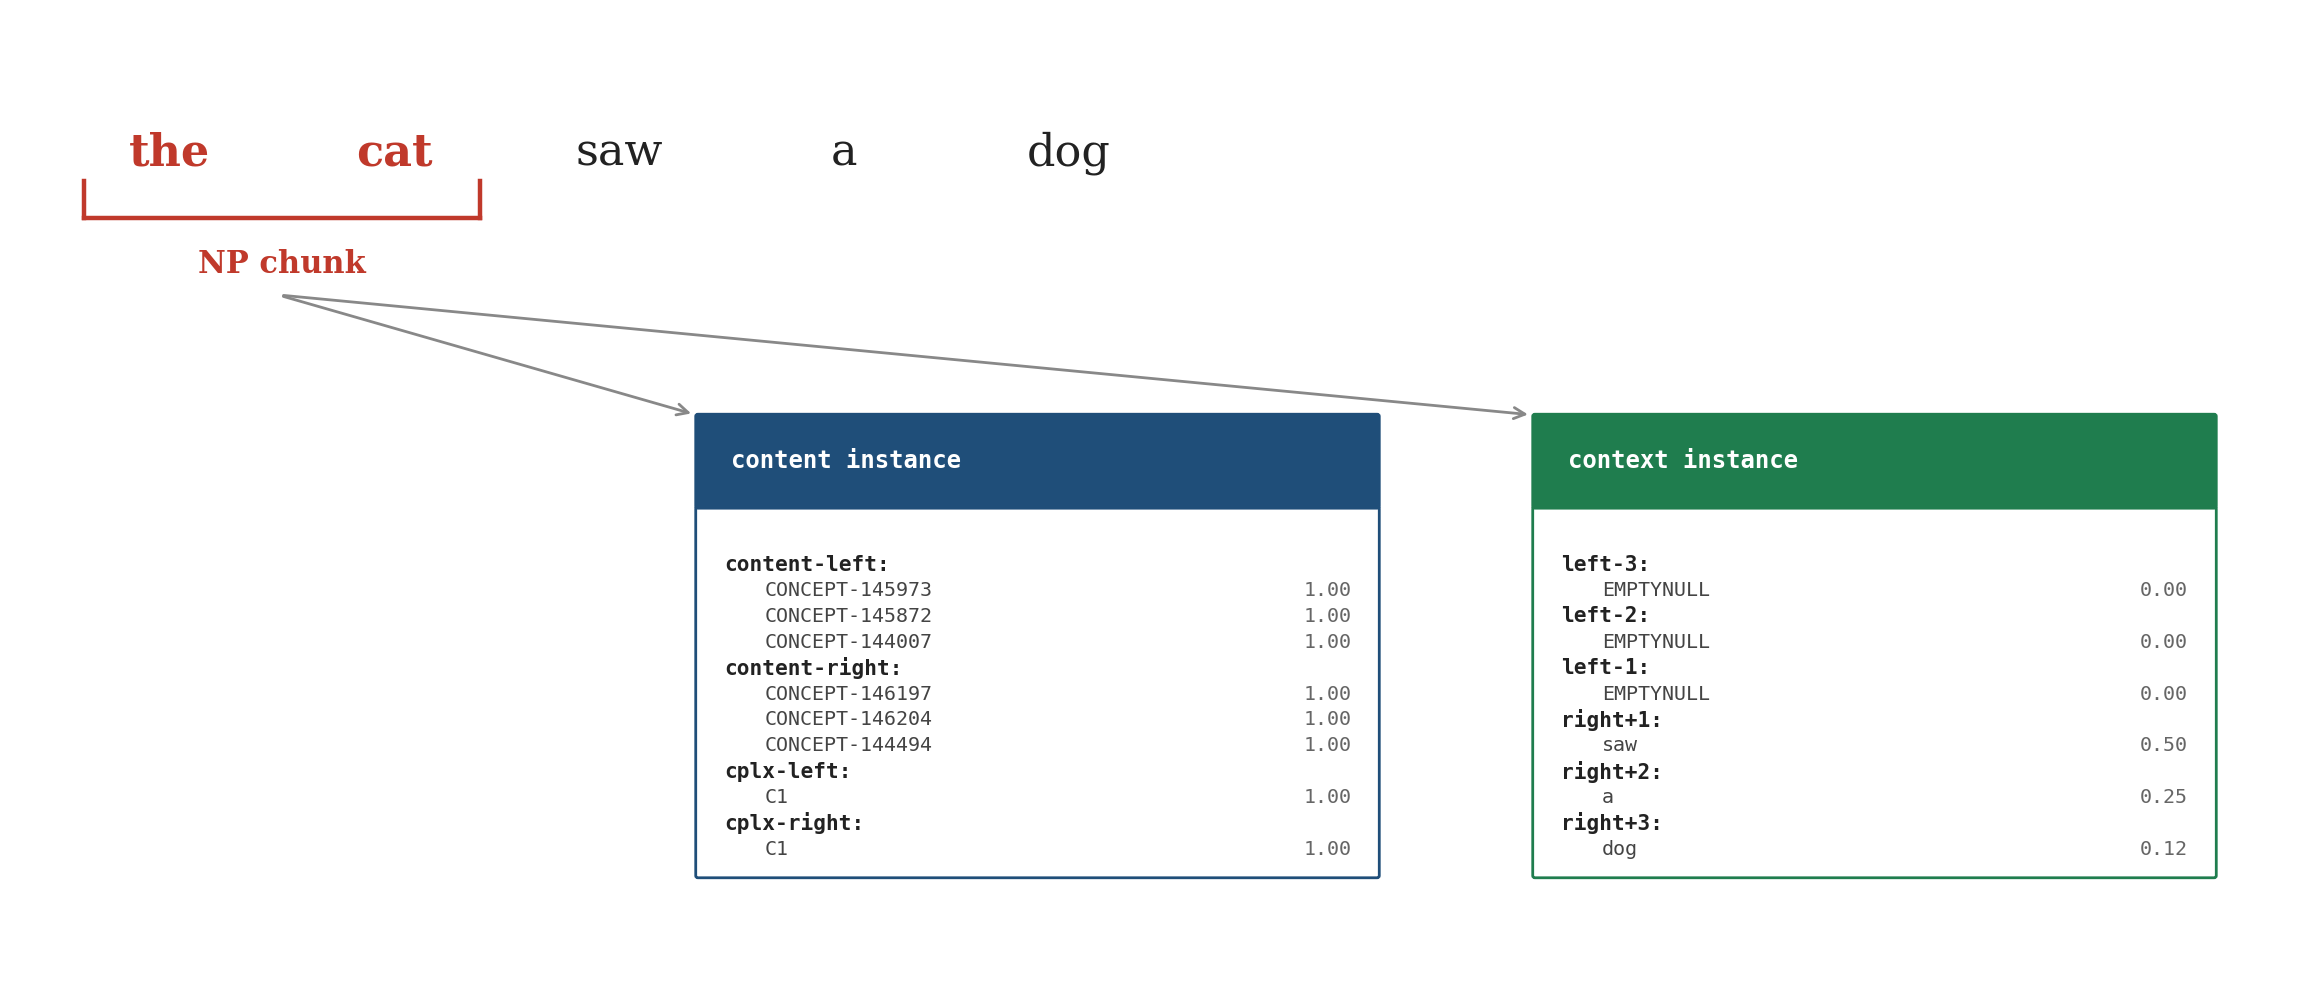
\includegraphics[width=0.95\textwidth]{graphics/instances.png}
\caption{A sample sentence with the noun-phrase chunk ``the cat'' highlighted, together with the content instance and context instance that \textsc{Trellis} constructs for it. The content instance names the chunk's two children (the determiner ``the'' on the left, the noun ``cat'' on the right). The context instance names the elements that flank the chunk in the input.}
\label{fig:instances}
\end{figure}

\subsection{Organization}

\textsc{Trellis} organizes long-term memory into two Cobweb taxonomies, as required by O3. Both inherit the commitments reviewed in Section~3.1, but they play complementary roles.

The content hierarchy classifies the content instances of composites and captures the regularities that govern how chunks are built. Because a composite's content instance refers to its children by identifiers drawn from the context hierarchy, similarity in the content hierarchy is grounded in similarity of parts in the context hierarchy. Inspection of a trained content hierarchy typically reveals that composites with structurally similar children --- for instance, an adjective phrase followed by a noun, and a determiner followed by a noun --- occupy nearby positions in the hierarchy, reflecting their shared role as constituents that can fill an NP slot.

The context hierarchy classifies the context instances of every element the system has encountered, treating each as a singleton defined by its surroundings. Every element has a context instance, so every element appears here; only composites also appear in the content hierarchy, which follows from R3. The context hierarchy is responsible for grouping elements that play interchangeable distributional roles: a noun and an adjective phrase, for instance, will be sorted together in the context hierarchy because they appear before the same kinds of right-neighbors and after the same kinds of left-neighbors. Figure~\ref{fig:hierarchies} shows a subtree of a trained content hierarchy alongside a subtree of the corresponding context hierarchy, and calls out the regions in which AdjP and N occupy the same context-hierarchy subtree while the recursive AdjP productions Adj+AdjP and the NP-internal Adj+N occupy the same content-hierarchy subtree.

\begin{figure}[t]
\centering
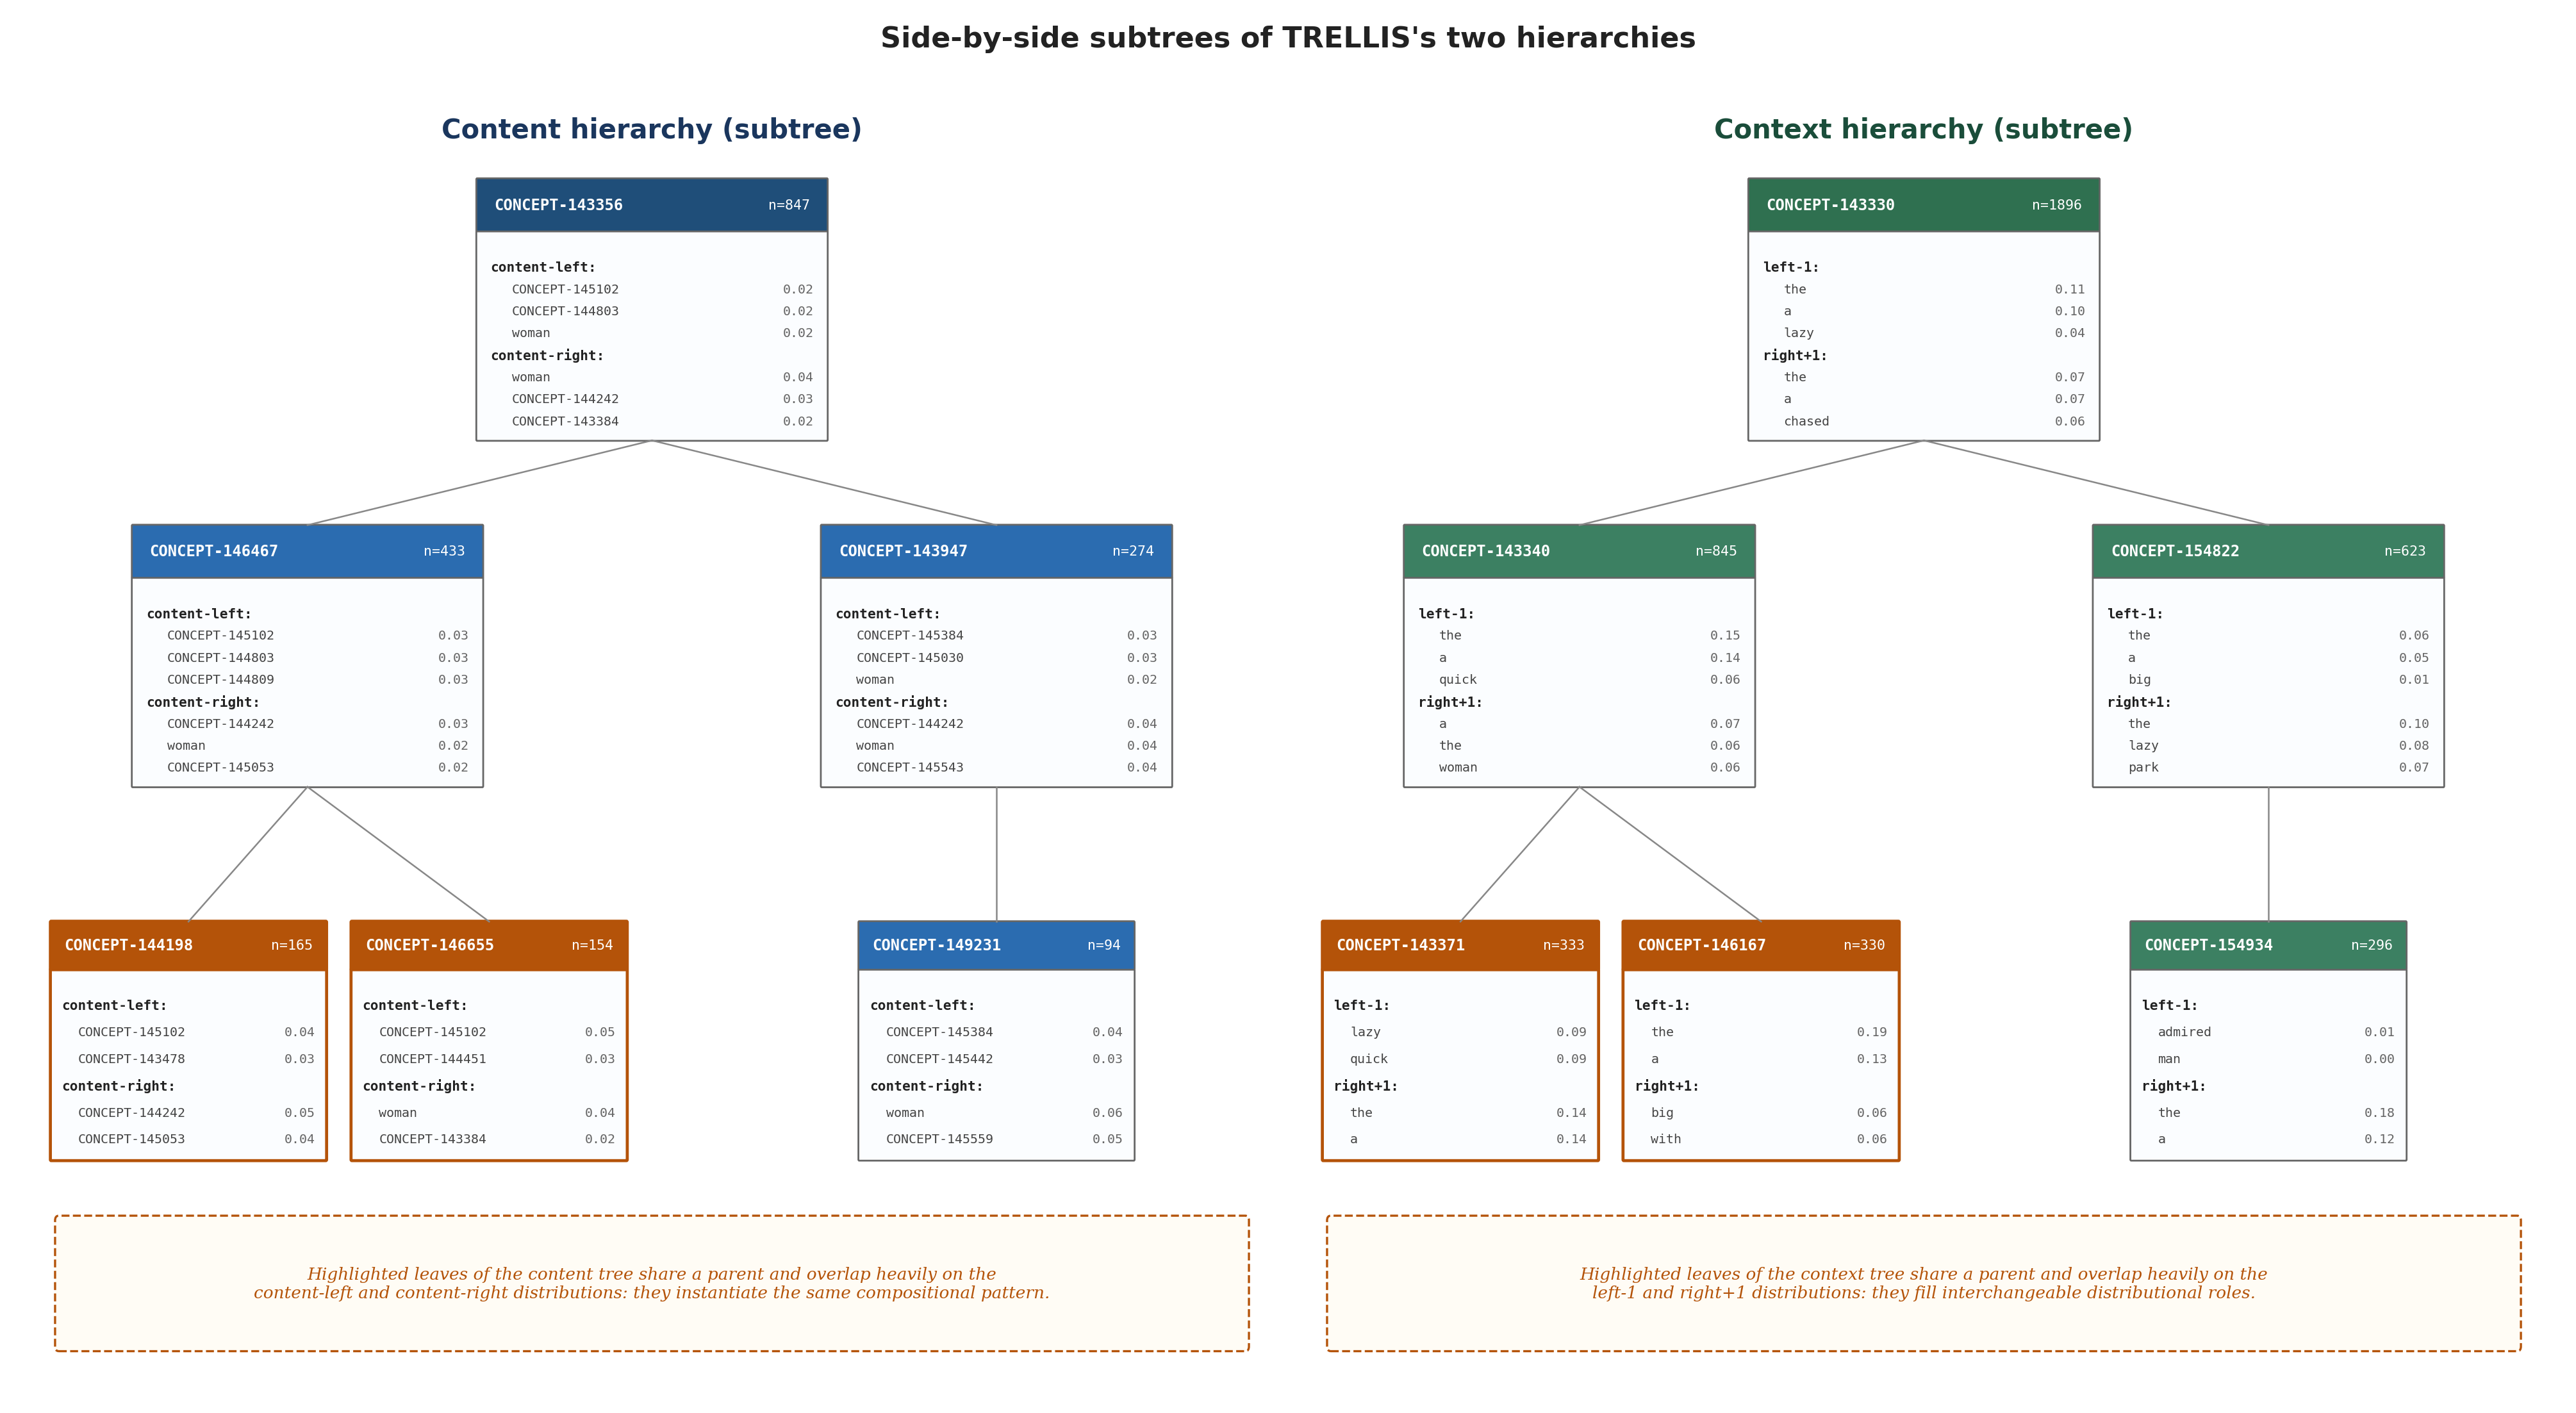
\includegraphics[width=0.95\textwidth]{graphics/hierarchies.png}
\caption{Subtrees of a trained content hierarchy (left) and context hierarchy (right). The two hierarchies organize the same elements along orthogonal dimensions: by what they are made of, and by what surrounds them. AdjP and N share a subtree in the context hierarchy because they fill interchangeable distributional roles; the recursive AdjP composite Adj+AdjP and the NP-internal Adj+N share a subtree in the content hierarchy because they share a compositional pattern.}
\label{fig:hierarchies}
\end{figure}

Alongside these two long-term structures sits a transient working structure: the partonomic parse tree for the current experience. The parse tree is a scratchpad on which \textsc{Trellis} accumulates its committed elaborations. Each of its nodes references the content concept and the context concept that classify it, allowing both hierarchies to score the parse as it grows and to absorb its nodes as they are committed.

\subsection{Performance}

\textsc{Trellis} realizes the performance commitments of postulates P1 through P10 as two complementary processes: parsing, which incrementally builds chunks from a given experience, and generation, which incrementally unpacks chunks back into primitives. The two are described in turn below; the exact formulas for the scoring, threshold, and sampling steps appear in Appendix~B.

\subsubsection{Parsing}

\textsc{Trellis} parses an input experience through a single performance loop, the procedural realization of P1 through P5. The loop consumes primitives and elaborates them into composites. At the start of a parse, the partonomic parse tree is initialized with the primitives of the input; these form the parse frontier from which the first elaboration begins, and the system operates on the frontier from this point on.

Each elaboration forms a candidate chunk for every adjacent pair of elements on the current frontier. A candidate is a hypothesized composite whose left and right children would be the paired elements. \textsc{Trellis} evaluates each candidate by routing its content instance through the content hierarchy and its context instance through the context hierarchy, yielding a content-recognition score and a context-recognition score that together express how well the candidate matches the chunks the system has consolidated. In the present implementation, the recognition scores are the root log-probabilities of the candidate's content and context instances in their respective hierarchies, which serve as monotonic proxies for the goodness-of-fit of the candidate to each hierarchy.

A recognition threshold then separates candidates the system can confidently call familiar from candidates that look like accidents of the current input. Candidates that fail are discarded; the highest-scoring survivor is committed as a new composite. Its two children are removed from the frontier, the composite takes their place, and the next elaboration begins from the updated frontier against an updated long-term memory whose new state is described in Section~4.4. The threshold itself is computed by a climbing-ancestor procedure that walks up the candidate's context-hierarchy path until it finds a level whose support exceeds a tuned minimum; a candidate passes when such a level exists, and fails when the procedure walks all the way to the root without finding one.

The loop repeats until no candidate passes the threshold. Parsing then terminates, and the remaining parse tree is the system's final account of the input: its frontier captures the chunks the system identified, and its internal structure captures the order in which they were assembled. Figure~\ref{fig:parsing-process} traces the loop on a representative sentence, showing how the frontier shrinks one elaboration at a time as composites are committed.

\begin{figure}[t]
\centering
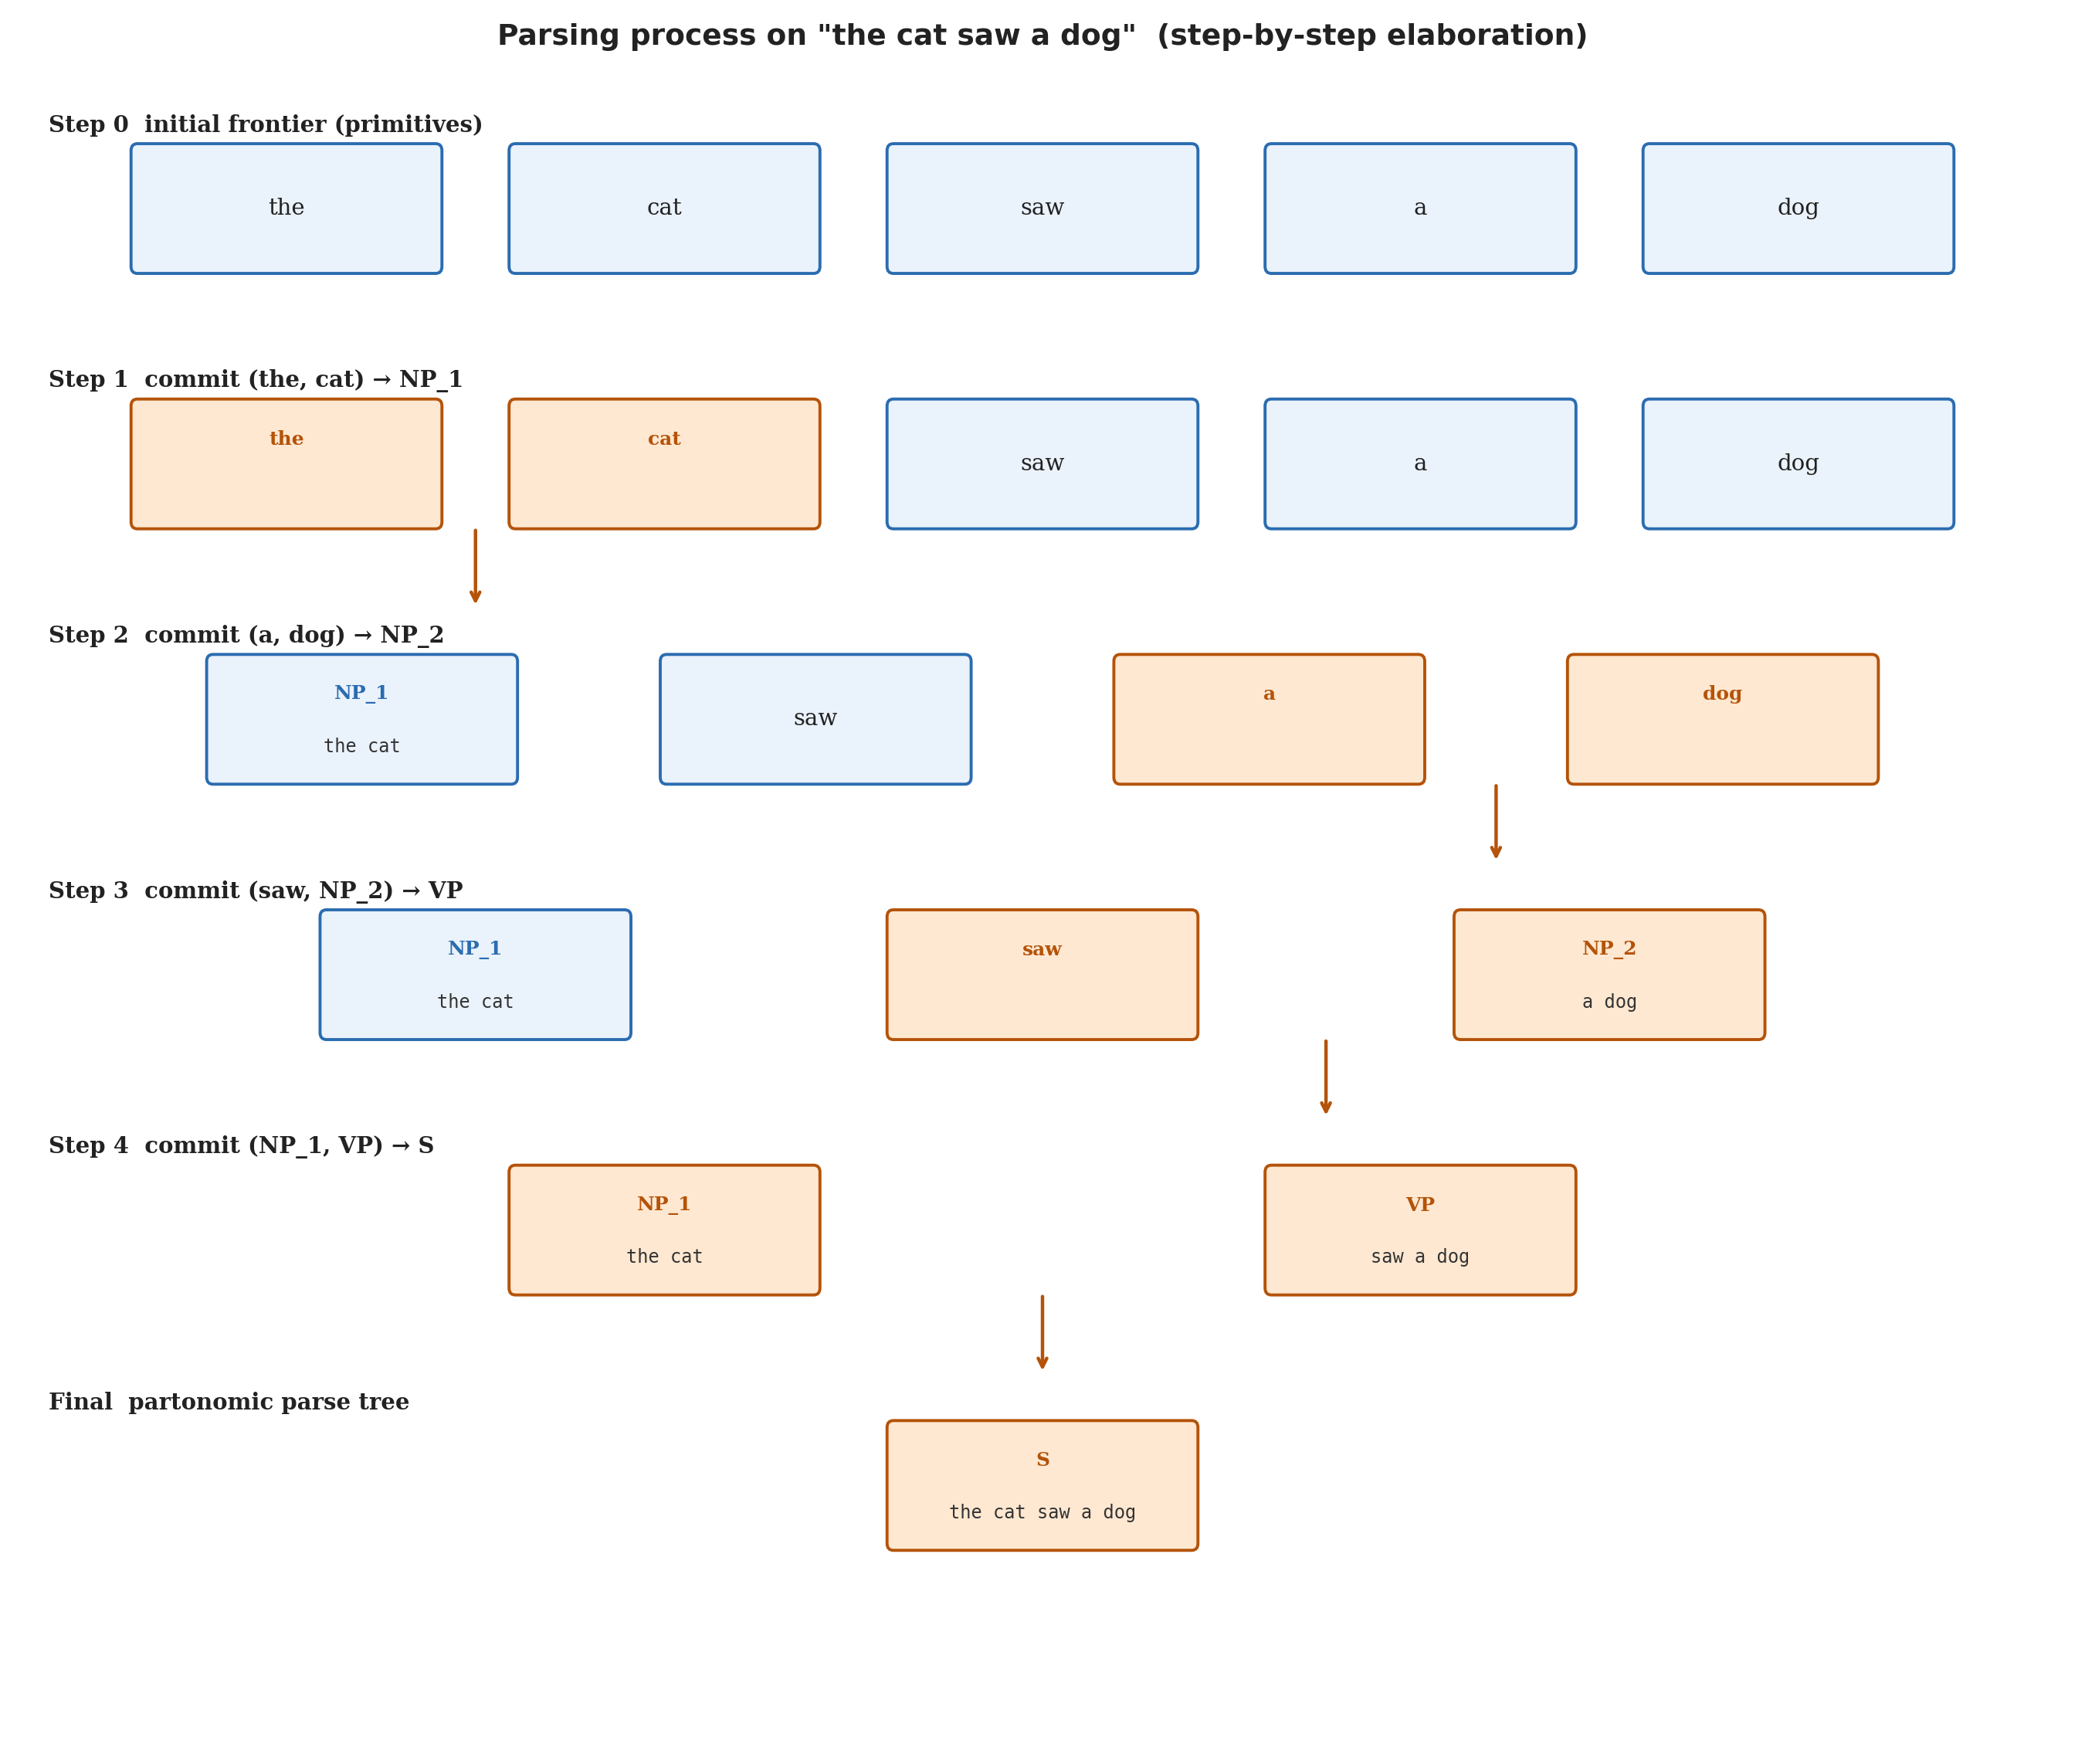
\includegraphics[width=0.95\textwidth]{graphics/parsing_process.png}
\caption{Step-by-step trace of \textsc{Trellis} parsing the sentence ``the cat saw a dog''. Each row shows the parse frontier after one elaboration; the highlighted boxes are the pair the system commits in that step, and the arrow points to the composite they become on the next row. After four elaborations, the frontier collapses to a single root composite that captures the full sentence.}
\label{fig:parsing-process}
\end{figure}

\subsubsection{Generation}

Generation inverts the parsing loop, as fixed by P6 through P10: where parsing elaborates upward from primitives to composites, generation expands downward from a composite seed back to primitives.

A generation step begins with a context-instance seed describing the element to be expanded. \textsc{Trellis} locates the leaf in the content hierarchy referenced by that seed, identifies the basic-level concept above it, and samples a fresh leaf from that concept --- a representative of the same class as the anchor, but not necessarily the anchor itself. If the sampled leaf is a primitive, the step returns it. Otherwise, its content instance names two children, each a reference into the context hierarchy; \textsc{Trellis} takes these as new seeds and recursively generates from each, producing the left and right subtrees of the composite being expanded.

The basic-level concept plays two roles. It fixes the level of abstraction from which the leaf is drawn, and it guarantees that the leaf comes from a class the system has actually consolidated rather than an idiosyncratic exemplar. Because the content children of each sampled leaf are already references into the context hierarchy, every expansion produces valid seeds for the next recursive call, and the procedure proceeds until every branch terminates at a primitive. In practice we have found that the basic level can be efficiently approximated by walking up the content hierarchy until the prior probability of the current concept exceeds a tuned threshold, an approximation that we describe in Appendix~B. Figure~\ref{fig:generation-process} traces the inversion on the same sentence, showing how a single seed expands downward through successive levels until every branch reaches a primitive.

\begin{figure}[t]
\centering
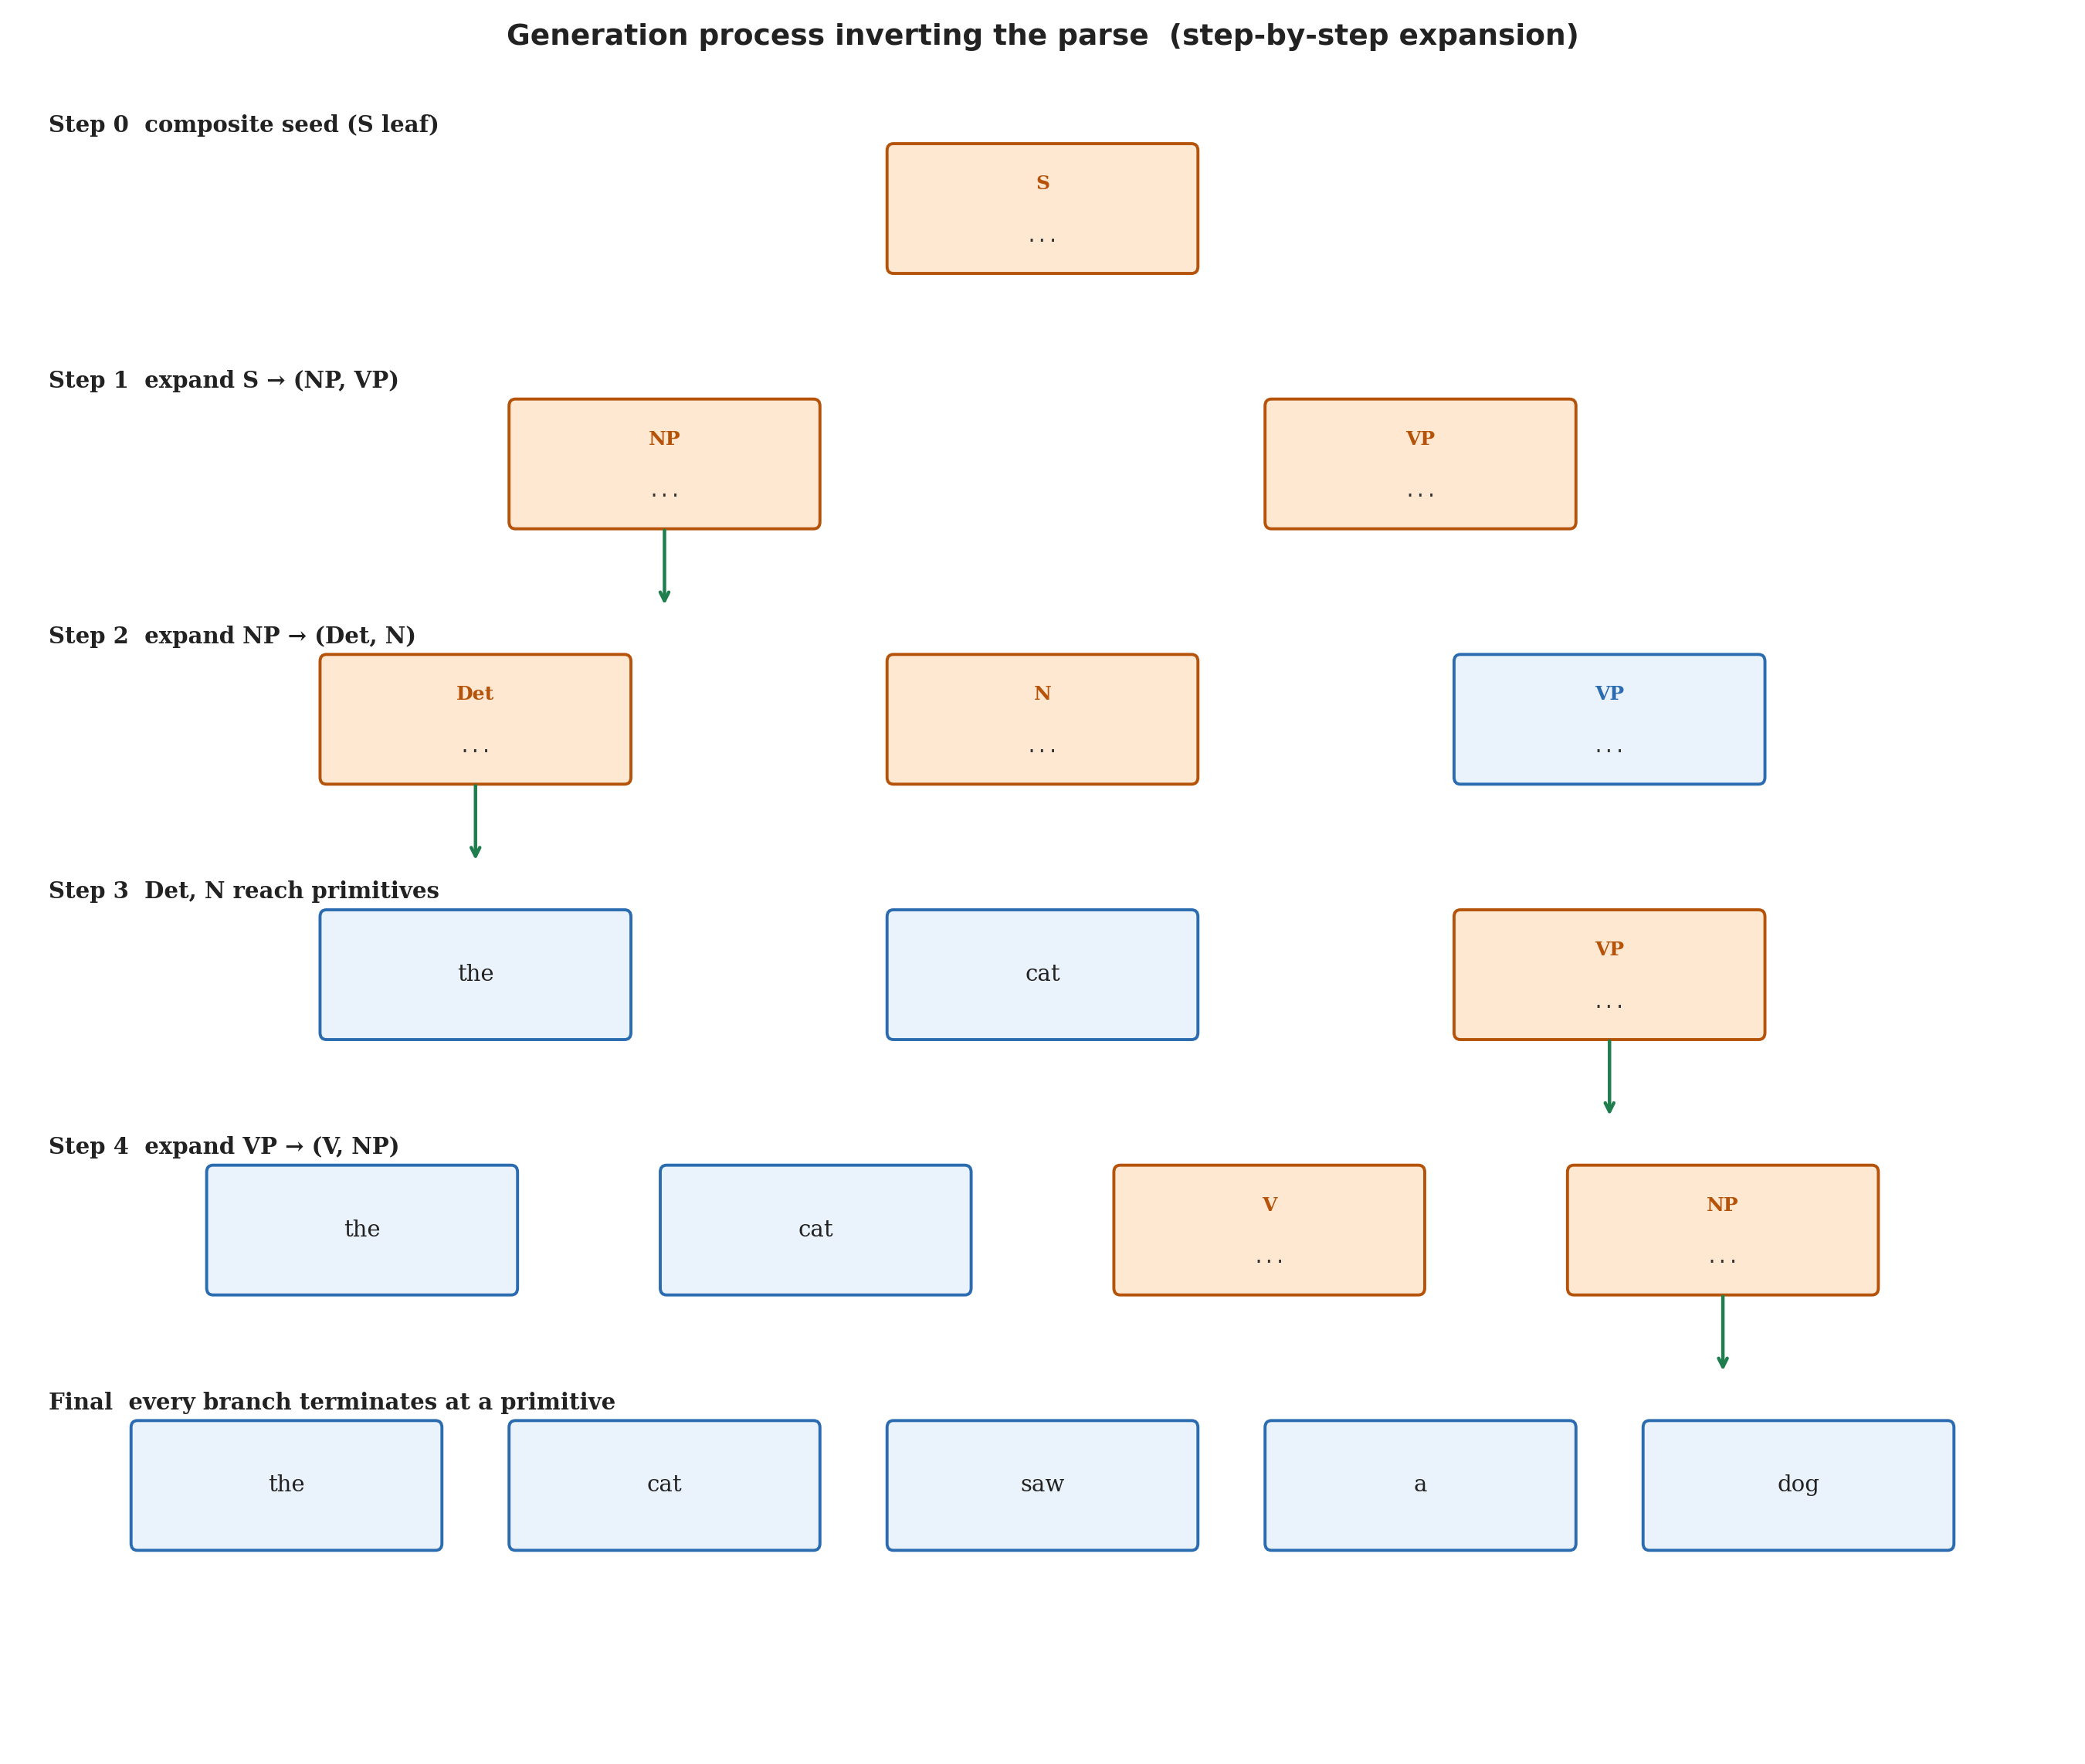
\includegraphics[width=0.95\textwidth]{graphics/generation_process.png}
\caption{Step-by-step trace of \textsc{Trellis} generating ``the cat saw a dog'' from a composite seed. Each row shows the partonomic frontier after one expansion; the highlighted box is the seed being expanded in that step, and the arrow points to the children it expands into on the next row. Generation terminates when every branch has reached a primitive.}
\label{fig:generation-process}
\end{figure}

\subsection{Learning}

Learning in \textsc{Trellis} is the absorption of parse-committed elaborations into the two long-term hierarchies. There is no separate training regime: every commit during the performance loop is followed immediately by an update to memory, so parsing and learning interleave one step at a time. This realizes L1.

When a composite is committed, \textsc{Trellis} sorts its content instance into the content hierarchy and its context instance into the context hierarchy, each via the standard Cobweb procedure of Section~3.1 (L2, L4). The two sorts run independently and in parallel. Primitives encountered during a parse are sorted into the context hierarchy alone, in accordance with L2, since they carry no content instance.

Restricting primitives to the context hierarchy keeps the content hierarchy compositional by construction: every leaf there is a composite whose children are valid references into the context hierarchy. This invariant is what makes the generation procedure of Section~4.3.2 well-defined --- sampling any content leaf yields two valid seeds rather than a malformed reference.

Because both hierarchies are updated immediately, candidates produced later in the same parse are scored against a memory that already reflects the chunks committed earlier. Performance and learning are tightly coupled: a composite committed near the start of an experience can shape the system's recognition of candidates near its end, and over repeated experiences the two hierarchies converge toward a shared organization of the chunks the system has come to recognize.

\subsection{Implementation Details}

The \textsc{Trellis} architecture is implemented in Python, with the underlying Cobweb hierarchies provided by a C++ extension. Both hierarchies are instances of the same Cobweb data structure, parametrized only by the attribute vocabulary they classify. The content hierarchy uses attributes for the left and right child identifiers along with a small set of complexity annotations that record the structural depth of the composite's children; the context hierarchy uses attributes that name the immediate left- and right-neighbors of the element being classified, plus optional surrounding-window attributes when richer context is available.

Two tuned parameters govern the system's behavior. The first is a uniform Cobweb prior $\alpha$, which controls the base-rate smoothing of R5 and was set to $1/V$ for tree alpha and to $1$ for basic-level computation, with $V$ the vocabulary size of the receiving hierarchy. The second is the recognition threshold, parameterized as a minimum context-hierarchy count $\tau$, which controls how readily a candidate is judged familiar. Both parameters and the exact form of every score, threshold, and sampling step appear in Appendix~B.

\section{Evaluation of \textsc{Trellis}}

The theory presented in Section~3 offers an account of how a chunking system might combine the categorical commitments of concept formation with the compositional commitments of chunking. A primary reason for implementing the theory in \textsc{Trellis} is to verify that the resulting system behaves as the theory predicts. In this section we report a sequence of experiments on synthetic context-free grammars of increasing complexity, demonstrating that \textsc{Trellis} can parse novel sentences with high accuracy, generate novel grammatical sentences from memory, learn incrementally from a small number of training sentences, and scale gracefully along both grammar complexity and terminal-vocabulary size. The full grammars used in these experiments are given in Appendix~A.

\subsection{Setup}

The empirical setup consists of three synthetic context-free grammars of increasing complexity, each instantiating a different point on the spectrum from minimal recursive structure to the kind of grammar one might use to model a fragment of English. TEST\_GRAMMAR\_SMALL admits sentences of the form ``$\text{NP}_{\text{Det+N}}\;\text{VP}_{\text{V}\;(\text{NP})}$'' with four nouns, four verbs, and two determiners. TEST\_GRAMMAR\_MED extends the small grammar with adjective phrases (AdjP), prepositional phrases (PP), and a transitive verb-phrase production V+NP+PP. TEST\_GRAMMAR\_LARGE further introduces relative clauses (RelClause) with relative pronouns (RelPro), producing a grammar whose sentences may contain center-embedded RelClauses with their own internal NP--VP structure. The complete productions and terminal lexicons are listed in Appendix~A.

For each grammar, we generated a corpus of derivation-annotated sentences: the small and medium grammars yielded 200 sentences each, and the large grammar yielded 400 sentences to compensate for its greater structural variety. The gold brackets for each sentence are obtained directly from the CFG derivation tree, with a fixed binarization convention (right-binary inside NP/PP/AdjP, flatten VP at the parent level, left-incremental at the S level) that matches the convention a human annotator would adopt. As an internal reference point we also computed metrics for a parser, denoted \emph{hollow ref}, that uses the same binarization convention applied to hand-annotated training trees. The hollow reference is not a competing system but a marker of what the binarization convention permits when the training data is fully labelled; comparing \textsc{Trellis} against it indicates how much of the achievable accuracy the unsupervised system recovers without any supervision.

We report five metrics: \emph{Parse F1}, the standard labelled bracketing F1 on test sentences; \emph{Exact-match}, the fraction of test sentences whose full parse tree matches gold; \emph{Step-pick}, the fraction of individual elaboration decisions in which \textsc{Trellis} picks the gold next-chunk; \emph{From-scratch grammaticality}, the fraction of sentences sampled from the trained system that are grammatical under the source grammar; and \emph{Generation novelty}, the fraction of sampled sentences that do not appear verbatim in the training corpus. All metrics are averaged over five training seeds per grammar.

\subsection{Final Parsing and Generation Metrics}

Table~\ref{tab:headline} reports the headline 5-seed results across the three grammars, alongside the hollow reference. On the small grammar, \textsc{Trellis} matches the hollow reference on step-pick (both at 99.2\%) and substantially exceeds it on parse F1 (98.8\% vs 92.9\%) and exact-match (96.0\% vs 82.6\%). Two of the five small-grammar seeds reach a perfect 100\% on all parse metrics. This indicates that when the grammar is tight enough that the binarization convention is unambiguous, \textsc{Trellis} recovers the gold brackets almost exactly --- entirely without supervision.

\begin{table}[t]
\centering
\caption{Five-seed mean ± standard deviation of \textsc{Trellis}'s parsing and generation metrics across the three synthetic grammars, with the hollow reference parser shown for context. From-scratch grammaticality and novelty are reported on sentences sampled from the trained system after the final training pass.}
\label{tab:headline}
\begin{tabular}{lrrrr}
\toprule
Metric & Hollow ref & SMALL & MED & LARGE \\
\midrule
Parse F1 & 92.9\% & \textbf{98.8 ± 1.1\%} & 85.5 ± 7.5\% & 85.8 ± 5.2\% \\
Exact-match & 82.6\% & \textbf{96.0 ± 3.4\%} & 64.5 ± 11.9\% & 55.0 ± 13.8\% \\
Step-pick & 99.2\% & \textbf{99.2 ± 0.8\%} & 95.8 ± 3.2\% & 95.8 ± 1.4\% \\
From-scratch grammaticality & 100\% & 100\% & 100\% & 100\% \\
Generation novelty & --- & 46\% & 53\% & 67\% \\
\bottomrule
\end{tabular}
\end{table}

On the medium and large grammars, \textsc{Trellis}'s parse F1 lands roughly seven percentage points below the hollow reference. We trace the gap to two sources, both of which we examine in the next subsection. The first is \emph{training-induced drift}: as more sentences are absorbed into memory, the content hierarchy begins to specialize, and previously-reliable basic-level concepts become harder to recover. The second is a residual attachment ambiguity in the large grammar's RelClause productions, which accounts for the 12.6-point exact-match gap on TEST\_GRAMMAR\_LARGE; this is the only structural ambiguity in our corpora that resists greedy unsupervised parsing.

Step-pick remains above 95\% across all three grammars, indicating that even when the system makes occasional whole-parse mistakes, the great majority of its individual elaboration decisions remain correct. From-scratch generation grammaticality is 100\% across all grammar sizes, demonstrating that the generation procedure of Section~4.3.2, when seeded from a trained memory, never produces a sentence outside the source grammar. Generation novelty ranges from 46\% to 67\% across grammar sizes, with the larger grammars producing more novel sentences in proportion to their richer combinatorial space; this indicates that the generation procedure is not merely retrieving training sentences but is composing novel grammatical structures from generalized chunks. Figure~\ref{fig:generation-curves} reports both metrics as functions of the number of training sentences, with all three grammars overlaid on a common axis.

\begin{figure}[t]
\centering
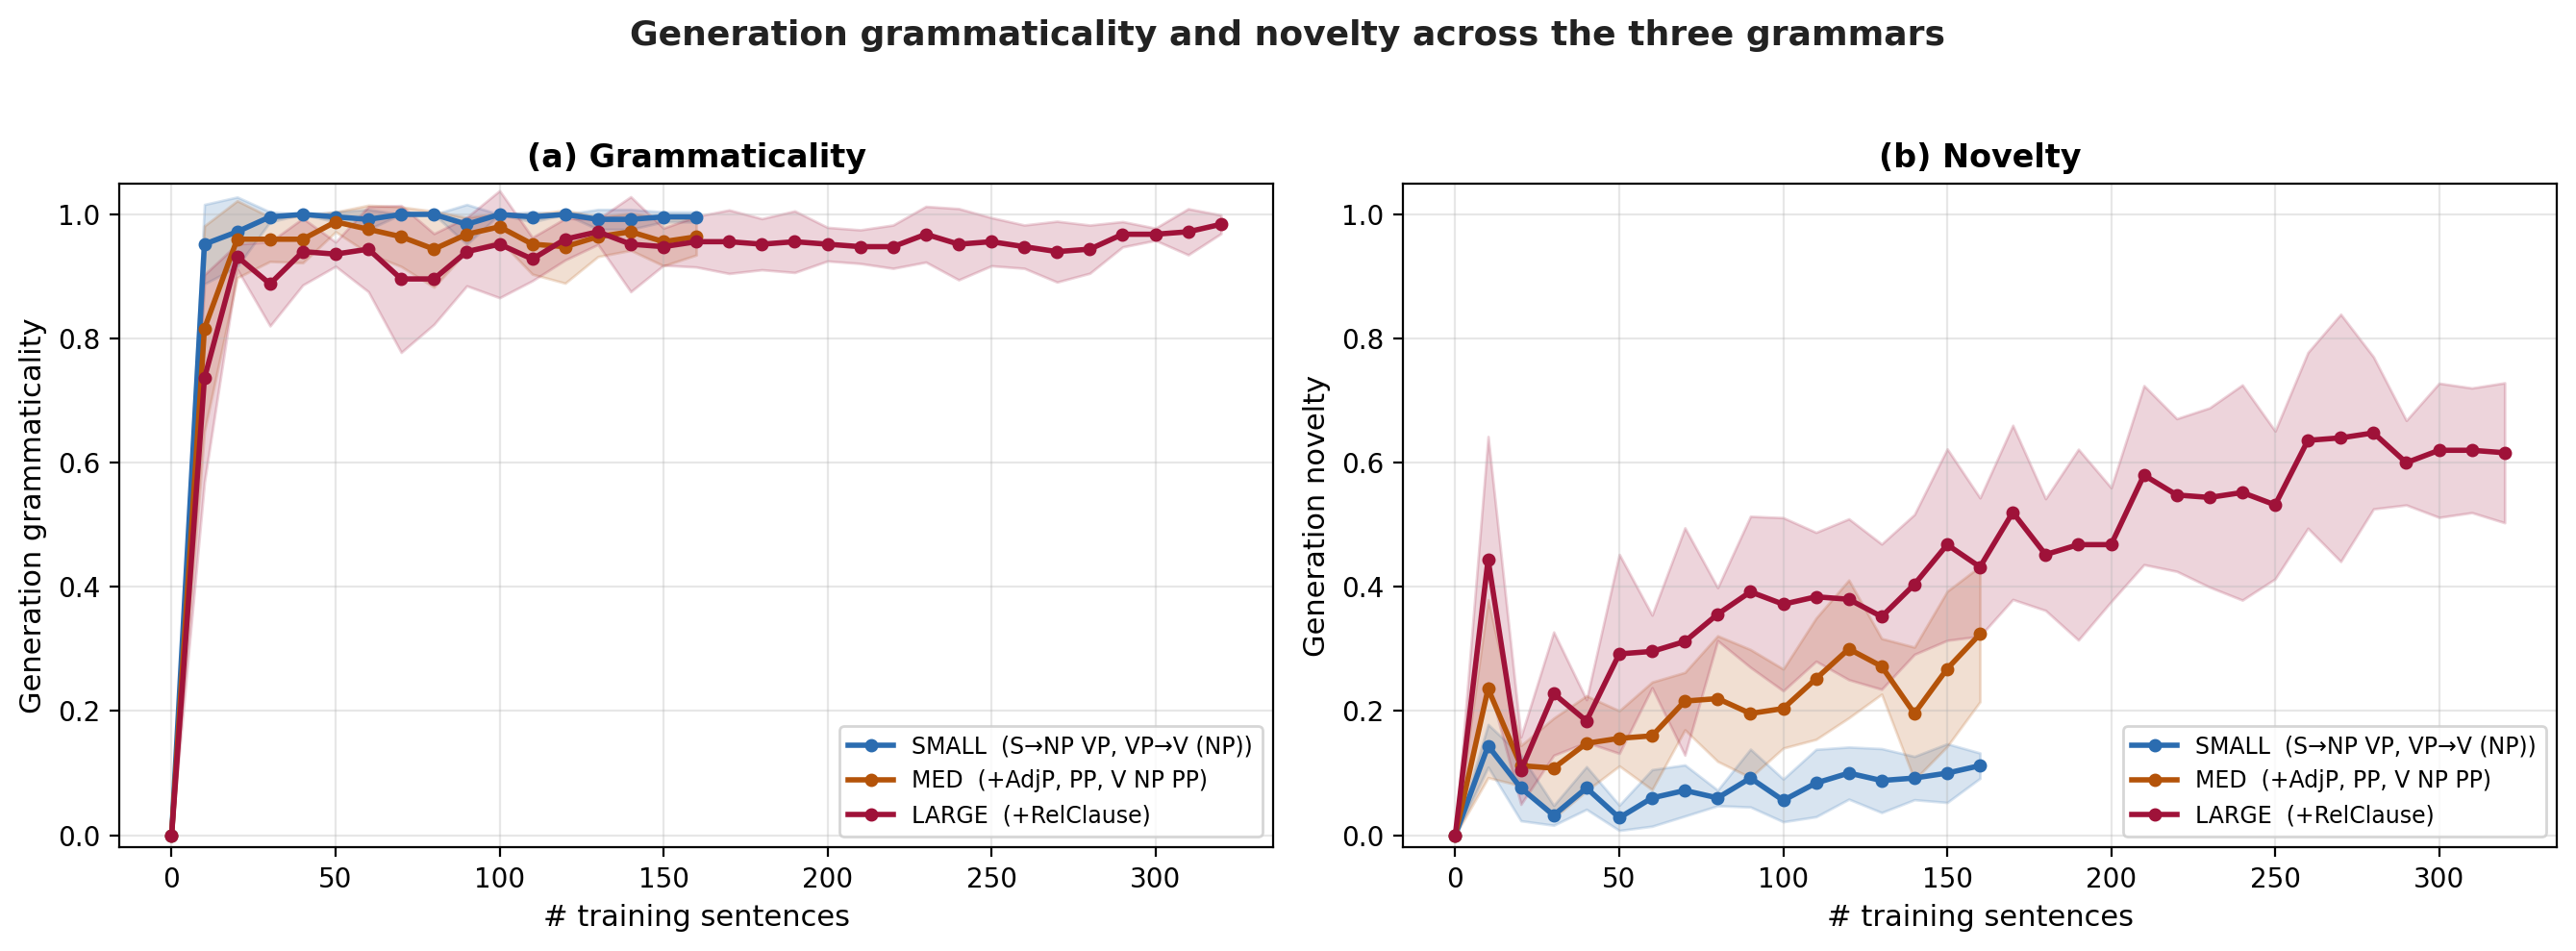
\includegraphics[width=0.95\textwidth]{graphics/generation_curves.png}
\caption{Generation grammaticality (left) and generation novelty (right) as functions of training-corpus size, overlaid for the three synthetic grammars. Mean ± standard deviation across five training seeds. Grammaticality saturates near $1.0$ on every grammar within the first few dozen training sentences; novelty rises monotonically and scales with grammar complexity, reflecting the larger combinatorial space available to the chunk-replay procedure on richer grammars.}
\label{fig:generation-curves}
\end{figure}

\subsection{Learning Curves and Error Analysis on the Medium Grammar}

To examine how the system's behavior changes with the size of its training corpus, we ran an incremental-training protocol that evaluates the system every ten training sentences on the medium grammar. Figure~\ref{fig:learning-curves} reports the resulting learning curves alongside a GRIDS-style decomposition of parse errors into \emph{errors of omission} (gold brackets the system failed to predict) and \emph{errors of co-mission} (system-predicted brackets that are not in gold). The two error categories together capture the standard precision/recall tradeoff in parsing, and presenting them side-by-side makes the dynamics of the parse-F1 curve interpretable.

\begin{figure}[t]
\centering
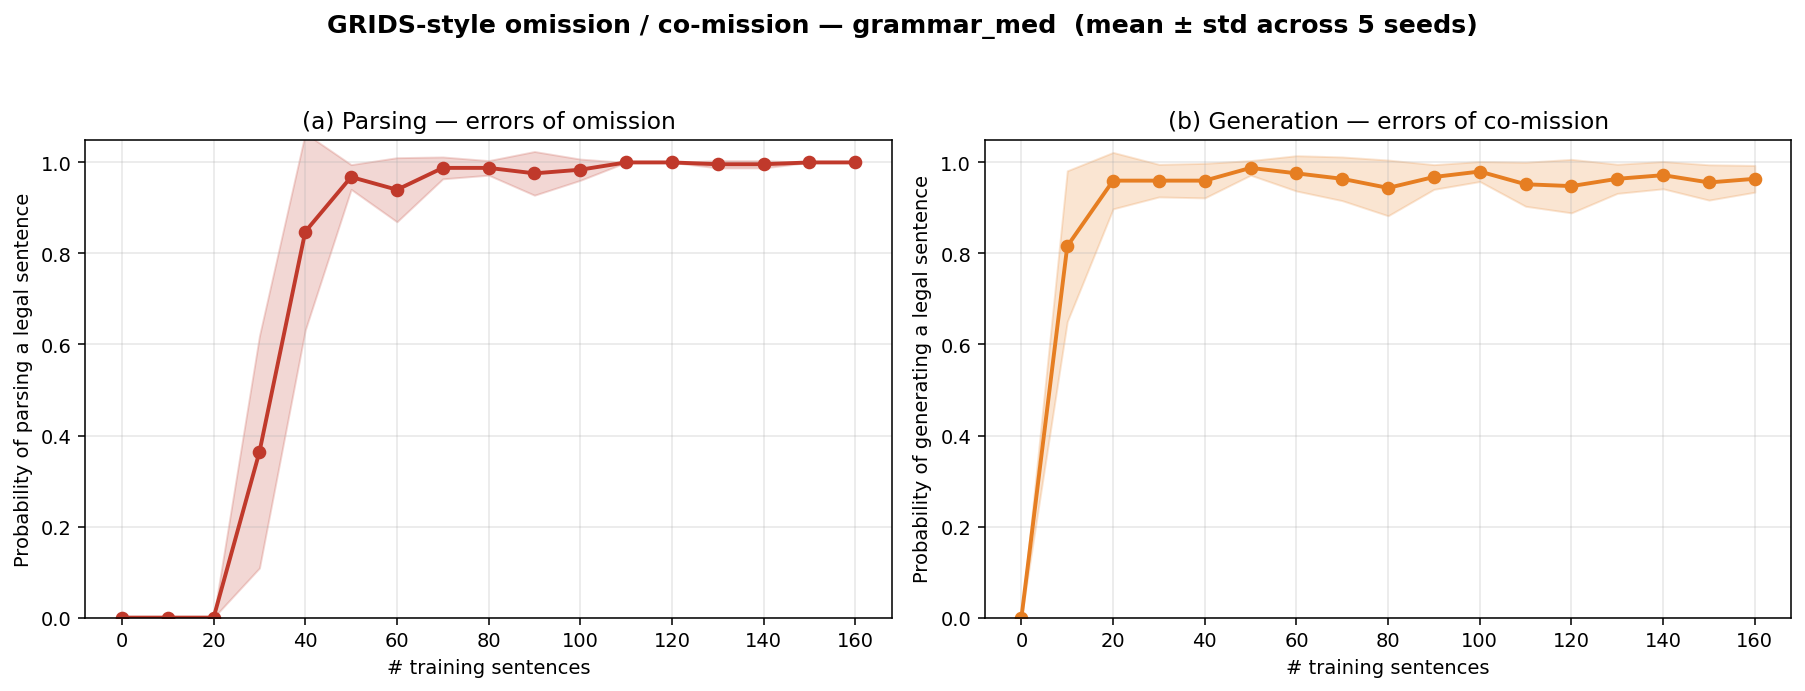
\includegraphics[width=0.95\textwidth]{graphics/learning_curves_med.png}
\caption{Learning curves on TEST\_GRAMMAR\_MED. The panels report parse F1, generation grammaticality, and generation novelty alongside the GRIDS-style decomposition of parsing errors into errors of omission (gold brackets missed) and co-mission (predicted brackets not in gold). Parse F1 peaks around 30--50 training sentences and drifts down thereafter as omission errors gradually rise; co-mission errors remain near floor throughout.}
\label{fig:learning-curves}
\end{figure}

Two patterns are visible. First, parse F1 rises sharply over the first 30--50 sentences, reaching a peak above 88\% on the medium grammar, then drifts down by roughly 10--15 points over the next 150 sentences. The omission/co-mission decomposition makes the direction of the drift legible: co-mission errors stay close to floor throughout the run, while omission errors gradually climb. \textsc{Trellis} does not begin asserting spurious brackets as it trains; it begins failing to assert correct ones. This pattern is consistent with what one would expect from a system that uses basic-level concepts as its categorical anchors and a fixed recognition threshold to gate commitments. As the content hierarchy grows, the basic-level frontier moves downward, and previously-confident candidates start failing the threshold because their context-hierarchy support no longer dominates the noise of finer-grained distinctions made elsewhere in the tree. The fix this pattern points to is not a richer scoring function but an \emph{adaptive} threshold that tracks the hierarchies' growth; we return to this in Section~7.

Second, generation grammaticality remains at 100\% throughout the run, and generation novelty rises monotonically as more chunks accumulate. The two generation metrics are essentially decoupled from the drift in parse F1: training-induced drift damages \textsc{Trellis}'s ability to \emph{recognize} familiar chunks under threshold, but it does not damage the chunks that have already been consolidated, so generation from the existing memory continues to produce grammatical structures. This is precisely the asymmetry one would expect under the postulates: parsing depends on a per-candidate threshold judgment, while generation depends only on the structural invariants of the content hierarchy, which L2 and L3 keep well-formed by construction.

\subsection{Generalization Across Grammar Complexities}

Figure~\ref{fig:comparison-grammar} reports a five-seed GRIDS-style overlay of \textsc{Trellis}'s parsing and generation behavior across the three grammars as a function of training-corpus size. The left panel shows errors of \emph{omission} on parsing, measured as the probability of finding any legal parse for a held-out sentence; the right panel shows errors of \emph{co-mission} on generation, measured as the probability that a sampled sentence is grammatical under the source grammar. Higher values in each panel correspond to fewer errors of the respective kind. The mean and the shaded standard-deviation band are computed over five training seeds.

\begin{figure}[t]
\centering
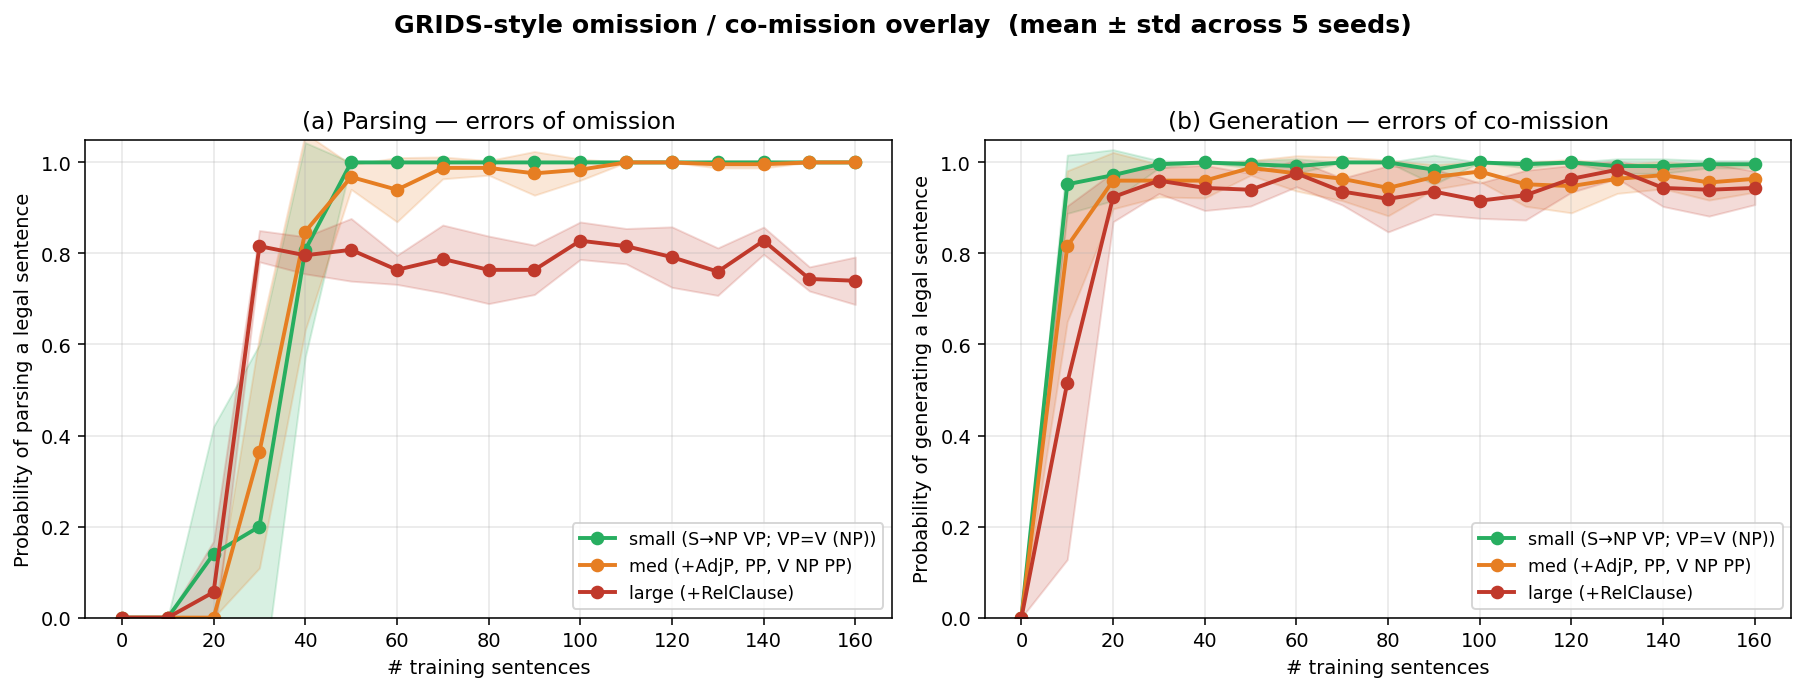
\includegraphics[width=0.95\textwidth]{graphics/grids_grammar_sweep.png}
\caption{GRIDS-style omission/co-mission overlay across the three synthetic grammars, plotted against training-corpus size. Left: probability of finding a legal parse on a held-out sentence (errors of omission). Right: probability of generating a grammatical sentence from the trained system (errors of co-mission). Mean ± standard deviation across five training seeds.}
\label{fig:comparison-grammar}
\end{figure}

Two patterns are visible. On parsing, the omission curve for the SMALL grammar reaches the asymptote of $1.0$ within roughly 30 training sentences and stays there for the rest of the run; the MED and LARGE grammars approach the asymptote more slowly and settle at $0.80$--$0.85$ by the end of training. The systematic ranking of the three grammars by grammar size --- SMALL above MED above LARGE --- reflects the system's increasing difficulty in finding legal parses as RelClauses and AdjP recursion add structural ambiguity that the greedy elaboration loop cannot always resolve. On generation, the co-mission curve climbs rapidly to $1.0$ on every grammar and remains there throughout training. The asymmetry between the two panels is the same one we observed on the medium grammar in Section~5.3: training-induced drift accumulates omissions but not co-missions, and the asymmetry holds across the full grammar sweep. Taken together, the overlay shows a system whose strengths and failure modes scale predictably along the complexity axis: it is best on tight grammars, gradually loses parsing recall as ambiguity increases, but continues to produce well-formed structures from memory throughout.

\subsection{Generalization Across Terminal Vocabularies}

A second axis along which a chunking system can be stressed is the size of the terminal vocabulary. A larger lexicon means more primitives, fewer repetitions of each primitive in the training corpus, and weaker context-hierarchy support for each individual primitive. Figure~\ref{fig:comparison-terminal} reports the same GRIDS-style overlay used in the previous subsection, this time across three terminal-vocabulary sizes (low: 11 terminals; medium: 22 terminals; high: 39 terminals) at fixed grammatical complexity --- the productions are held constant and only the number of terminals per part of speech varies.

\begin{figure}[t]
\centering
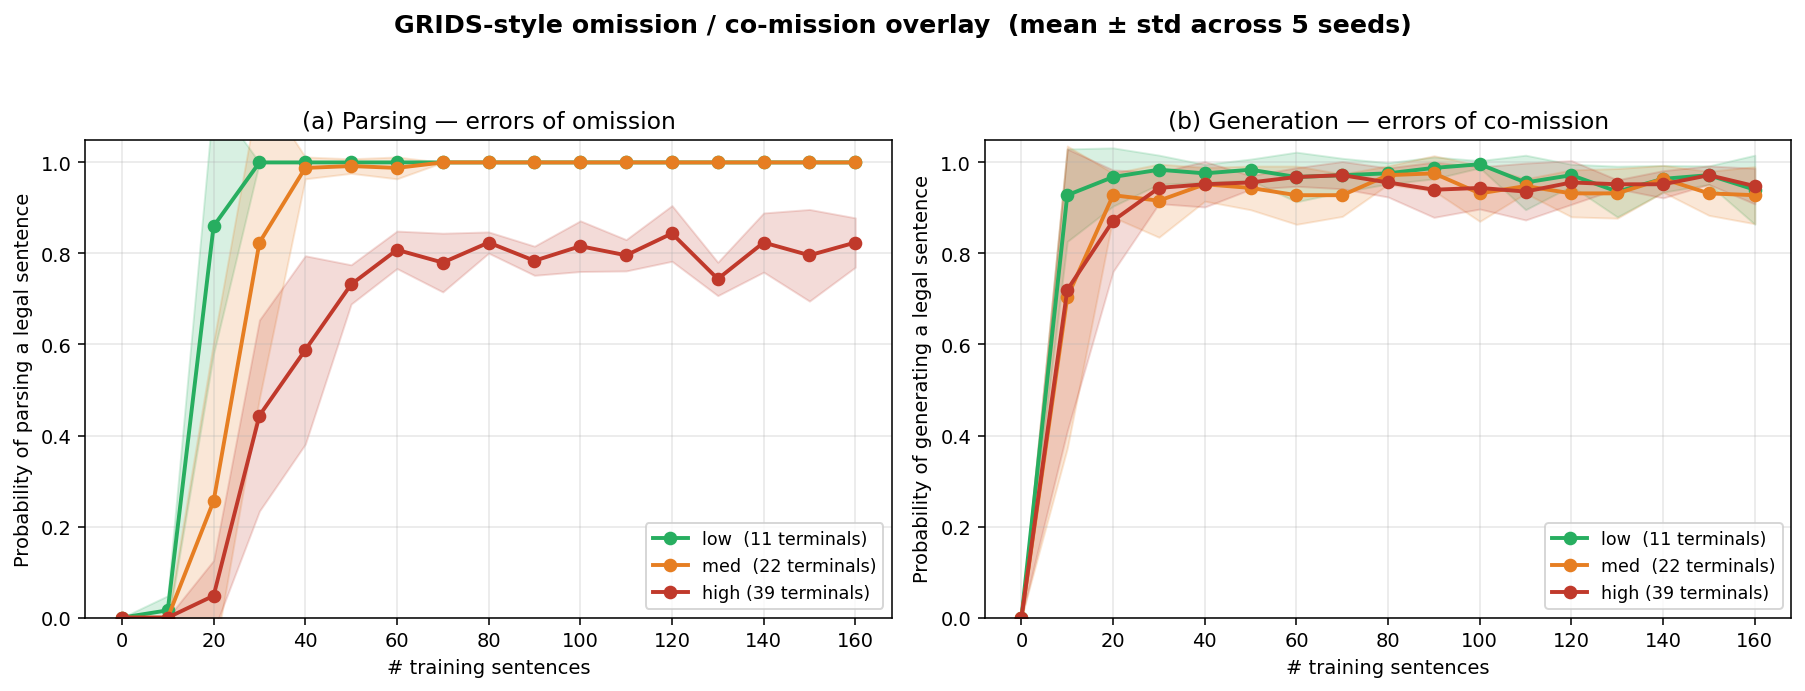
\includegraphics[width=0.95\textwidth]{graphics/grids_terminal_sweep.png}
\caption{GRIDS-style omission/co-mission overlay across three terminal-vocabulary sizes at fixed grammatical complexity, plotted against training-corpus size. Left: probability of finding a legal parse on a held-out sentence (errors of omission). Right: probability of generating a grammatical sentence from the trained system (errors of co-mission). Mean ± standard deviation across five training seeds per vocabulary size.}
\label{fig:comparison-terminal}
\end{figure}

\textsc{Trellis}'s parsing behavior is approximately stable across the terminal sweep: the omission curves for the low, medium, and high vocabularies all asymptote to roughly the same level, and the spread between them is contained within the seed-to-seed standard-deviation bands. This stability is a direct consequence of the two-hierarchy organization. The context hierarchy groups distributional equivalents (nouns with nouns, verbs with verbs), so even when a particular terminal appears only a handful of times in the training corpus, the context-hierarchy basic level above it inherits the strong support of its part-of-speech siblings, and the climbing-ancestor threshold therefore still passes for the chunks that use it. Without the context hierarchy, a system relying only on a content-hierarchy match would degrade sharply at high vocabulary sizes; with both hierarchies in concert, the system remains robust to the vocabulary expansion. The generation co-mission curves likewise reach $1.0$ across all three vocabulary sizes, confirming that generation grammaticality is preserved under vocabulary growth for the same structural reason we identified in Section~5.3.

\subsection{Discussion}

Taken together, these experiments establish four points. First, \textsc{Trellis} recovers gold brackets with high accuracy across grammars of varying complexity, matching the hollow reference on the small grammar and remaining within a few percentage points on the medium and large grammars --- entirely without supervision. Second, \textsc{Trellis} produces 100\% grammatical sentences from scratch on all three grammars and across the terminal-vocabulary sweep, with a substantial fraction of those sentences not appearing in the training corpus; generation composes from generalized chunks rather than retrieving memorized strings. Third, the system's behavior scales predictably along both grammar complexity and terminal-vocabulary size: parsing omission rises gradually with grammar complexity but is essentially unaffected by terminal-vocabulary growth, exactly the asymmetry the two-hierarchy organization predicts, since context-hierarchy generalization absorbs the per-terminal sparsity that would otherwise hurt parsing recall. Fourth, the GRIDS-style omission/co-mission decomposition --- both on the medium grammar in Section~5.3 and across the sweeps in Sections~5.4 and 5.5 --- reveals that \textsc{Trellis}'s errors are uniformly asymmetric: omissions accumulate where ambiguity or recognition-threshold tuning is hard, but co-missions stay near floor throughout, indicating that the chunks the system has consolidated remain well-formed even when the recognition step misses them under threshold.

The experiments also surface two failure modes that the theory predicts but does not currently resolve. The first is the training-induced drift in parse F1 just described, which we attribute to the absence of an adaptive recognition threshold. The second is residual attachment ambiguity in grammars with RelClause productions, where the greedy elaboration loop occasionally commits an incorrect early bracket that the rest of the parse cannot recover from. Both failure modes have natural treatments within the theory --- the first by adapting the threshold to the current state of the hierarchies, the second by introducing a limited form of look-ahead or backtracking --- and we discuss them in Section~7.

\section{Related Work}

The gap our theory aims to fill --- categorical generalization combined with compositional structure --- has been approached by several other lines of work, each with a different starting point and a different residual limitation. We review here the two lines that most directly attempt the same unification we propose: unified theories of concepts and chunks in the cognitive systems tradition, and grammar-induction systems in the machine learning tradition. The broader literatures on concept formation, chunking, and distributional language representation that motivate the unification were discussed in Section~2.

\subsection{Unified Theories of Concepts and Chunks}

The closest precursor to our proposal is \citet{langley-concepts-chunks}'s recent essay on concepts and chunks in cognitive systems, which surveys the parallel literatures on the two kinds of mental structure and argues that a unified theory should treat concept-hood and chunk-hood as two aspects of every representation rather than as two separate kinds of representation. That essay proposes a research agenda --- a set of representational, organizational, performance, and learning commitments that any unified system would need to satisfy --- but it does not commit to a specific implementation. Our theory can be read as one concrete instance of that agenda: a system in which every element carries both a categorical position in a taxonomy (its context-hierarchy classification) and a compositional position in a partonomy (its content-hierarchy classification), with the two hierarchies operating in tandem to support both recognition and reconstruction.

Earlier proposals in the same direction include the Matsakis system \citep{matsakis-cobweb}, which extended Cobweb in a related direction by introducing iterative additions to a script-like memory. That system shares with ours the use of Cobweb as a taxonomic substrate and the commitment to incremental, unsupervised learning, but it does not introduce the content--context distinction that lets our theory keep compositional and distributional structure separable. The convolutional Cobweb variant \citep{convolutional-cobweb} likewise pairs a chunking-style construction process with a classification-style hierarchy, but its construction process is fixed by the convolutional architecture rather than learned, and its setting (image classification) does not foreground the sequential, partonomic structure that drives our parsing loop.

\subsection{Grammar Induction}

The problem of inducing a grammar from a corpus of unannotated sentences has been studied in machine learning for decades and is, in effect, an instance of the gap our theory addresses: it asks for a system that can recover compositional structure (a grammar) from data using categorical generalization (the chunks that recur across sentences). \citet{wolff-grammar} introduced an early system that builds a phrase-structure grammar by repeatedly merging frequent adjacent pairs and generalizing the resulting categories; the procedure's two operations --- composition and generalization --- prefigure the two hierarchies we propose, though Wolff's system does not maintain them as separate structures. \citet{grids-langley-stromsten} introduced GRIDS, which performs Bayesian model selection over candidate grammars and frames grammar induction as a search through a discrete hypothesis space. GRIDS-style analysis methods, in particular the decomposition of parse errors into errors of omission and co-mission, have become the standard diagnostic tool for unsupervised parsing systems; we use that decomposition ourselves in Section~5.3 to characterize \textsc{Trellis}'s training-induced drift.

More recent work has explored neural approaches. \citet{diffusion-grammar} use a diffusion process over a latent partonomic representation to induce hierarchical structure from sentence corpora, and report that the noising--denoising loop naturally factors into chunk-construction and chunk-disassembly subprocesses analogous to the parsing and generation processes we describe. The neural setting trades off the discrete, incremental, postulate-driven character of our theory for the differentiable training and rich representation that come with continuous embeddings. The two approaches are complementary; we view the discrete, Cobweb-grounded route as the one most likely to support the postulate-level analysis that the cognitive systems community values, but the neural approach offers an attractive direction for scaling the basic two-process loop beyond the discrete attribute--value vocabulary our implementation currently uses.

\section{Conclusion and Future Work}

We have presented a theory of chunking that combines the categorical commitments of concept formation with the compositional commitments of the chunking tradition, and we have instantiated the theory in \textsc{Trellis}, a system that uses two Cobweb hierarchies as its taxonomic substrate to incrementally parse experiences into partonomic structures and to invert the same machinery for generation. The theory states a small set of postulates about how elements are represented, how memory is organized, how parsing and generation proceed, and how learning interleaves with both. The system instantiates each postulate concretely and produces parses whose accuracy, on three synthetic CFG benchmarks, ranges from 86\% to 99\% F1 with 100\% from-scratch generation grammaticality throughout.

The motivation for combining the two traditions is twofold. From the perspective of the concept-formation literature, the addition of a partonomic structure to a Cobweb-style hierarchy lifts the fundamental limitation that an instance has no parts; it enables Cobweb's incremental, unsupervised, generalizing machinery to apply to data whose structure is inherently compositional. From the perspective of the chunking literature, the addition of a taxonomic substrate gives the resulting system the categorical generality that pure chunking models lack; it lets a chunk recognize instances it has never literally seen, by virtue of those instances being sortable into the same basic-level concept as instances it has. The result is a system in which categories are defined in terms of shared chunks and chunks are defined by generalizations that appear through categories --- a mutual dependence that the literature reviewed in Section~2 has long argued is essential to any account of natural cognition.

A second contribution is methodological. By stating the theory as a set of postulates before describing the system that instantiates it, we make explicit which of \textsc{Trellis}'s behaviors are theoretical commitments and which are implementation choices. The recognition threshold, the basic-level approximation, and the binarization convention used by the parse procedure are all implementation choices, and the system would remain an instance of the same theory under a wide range of alternatives. The two-hierarchy organization, the content--context distinction, the inversion of parsing as generation, and the immediate absorption of parsed commits into long-term memory are theoretical commitments, and the system would no longer instantiate the theory if any of them were relaxed.

Several limitations of both the theory and the implementation deserve mention. First, the theory currently assumes a discrete and binary partonomic structure: every composite has exactly two children, and elements pair only with their immediate neighbors on the parse frontier. Real cognitive data exhibit richer partonomic structure, including $n$-ary chunks and non-adjacent dependencies, and extending the theory to handle these cases is a natural next step. Second, the implementation's recognition threshold is hand-tuned rather than adapted to the current state of the hierarchies, and we have argued in Section~5 that this is the proximate cause of the training-induced drift we observe on larger grammars. Replacing the fixed threshold with one that adapts to the hierarchies' growth would address this drift directly. Third, the implementation's parse loop is greedy: it commits the highest-scoring candidate at each step without considering whether a different early commit might enable a more accurate later parse. A limited form of look-ahead or backtracking would likely resolve the residual attachment ambiguities we observe on the large grammar.

Beyond these immediate refinements, the theory opens several avenues we find particularly worth exploring. One is the extension of the framework to non-linguistic domains. Nothing in the postulates of Section~3.2 is specific to language; the theory should apply equally to any domain in which experiences decompose into discrete elements that combine in regular ways, including event sequences, motor trajectories, and visual scenes. A second avenue is the scaling of the framework along the micro--macro axis: the same theory should let one parse letters into words, words into phrases, and phrases into sentences within a single taxonomic substrate, with the basic-level frontier shifting upward as more abstract chunks accumulate. A third avenue is the use of the system as a substrate for cumulative learning, in which chunks acquired in one experience become primitives for the next, recapitulating the piecemeal acquisition that \citet{langley-concepts-chunks} argues is characteristic of human learning.

The unification we have proposed --- categories defined by shared chunks, chunks defined by category-grounded generalization --- is one that the cognitive systems literature has gestured at for decades but has rarely committed to in implementation. We hope that the postulate-driven presentation of the theory and the empirical validation of \textsc{Trellis} together establish the unification as a viable foundation for further work on chunking, concept formation, and the structures that mediate between them.

\begin{acknowledgements}
\noindent
Shoutout to Zekun, Chris, friends at Teachable AI Lab etc etc etc
\end{acknowledgements}

\vspace{-0.25in}

{\parindent -10pt\leftskip 10pt\noindent
\bibliographystyle{cogsysapa}
\bibliography{main}

}

\appendix

\section{The Synthetic Grammars}
\label{app:grammars}

This appendix lists the productions and terminal lexicons of the three synthetic context-free grammars used in Section~5. Each grammar is presented in standard CFG form, with nonterminals in capitalized form and terminals in lowercase. Sentences are derived by selecting uniformly at random from the right-hand-side alternatives of each production.

\paragraph{TEST\_GRAMMAR\_SMALL.}
The smallest grammar has only a determiner-noun NP and a transitive or intransitive VP.

\begin{center}
\begin{tabular}{l@{\quad$\rightarrow$\quad}l}
\toprule
S    & NP VP \\
NP   & Det N \\
VP   & V NP \(\mid\) V \\
Det  & the \(\mid\) a \\
N    & dog \(\mid\) cat \(\mid\) man \(\mid\) woman \\
V    & runs \(\mid\) sees \(\mid\) likes \(\mid\) chases \\
\bottomrule
\end{tabular}
\end{center}

\paragraph{TEST\_GRAMMAR\_MED.}
The medium grammar adds an adjective phrase (with a recursive Adj-AdjP production and an empty alternative), prepositional phrases, and a transitive V+NP+PP verb-phrase production.

\begin{center}
\begin{tabular}{l@{\quad$\rightarrow$\quad}l}
\toprule
S    & NP VP \\
NP   & Det AdjP N \(\mid\) Det N \\
AdjP & Adj AdjP \(\mid\) Adj \(\mid\) $\varepsilon$ \\
VP   & V NP \(\mid\) V NP PP \(\mid\) V \\
PP   & P NP \\
Det  & the \(\mid\) a \\
N    & cat \(\mid\) dog \(\mid\) man \(\mid\) woman \(\mid\) park \(\mid\) telescope \\
Adj  & big \(\mid\) small \(\mid\) red \(\mid\) quick \(\mid\) lazy \\
V    & saw \(\mid\) liked \(\mid\) chased \(\mid\) found \(\mid\) admired \\
P    & with \(\mid\) in \(\mid\) on \(\mid\) under \\
\bottomrule
\end{tabular}
\end{center}

\paragraph{TEST\_GRAMMAR\_LARGE.}
The large grammar adds relative clauses with relative pronouns and removes the empty AdjP alternative. The NP production is weighted toward the simpler Det+N and Det+AdjP+N alternatives to keep RelClause sentences from dominating the corpus.

\begin{center}
\begin{tabular}{l@{\quad$\rightarrow$\quad}l}
\toprule
S         & NP VP \\
NP        & Det N \(\mid\) Det AdjP N \(\mid\) Det N RelClause \(\mid\) Det AdjP N RelClause \\
VP        & V NP \(\mid\) V NP PP \(\mid\) V PP \\
AdjP      & Adj \(\mid\) Adj AdjP \\
RelClause & RelPro VP \\
PP        & P NP \\
Det       & the \(\mid\) a \(\mid\) this \(\mid\) that \\
N         & book \(\mid\) boy \(\mid\) girl \(\mid\) teacher \(\mid\) robot \(\mid\) apple \\
Adj       & tall \(\mid\) curious \(\mid\) blue \(\mid\) ancient \(\mid\) friendly \\
RelPro    & who \(\mid\) that \(\mid\) which \\
V         & saw \(\mid\) liked \(\mid\) chased \(\mid\) carried \(\mid\) read \(\mid\) admired \\
P         & with \(\mid\) without \(\mid\) near \\
\bottomrule
\end{tabular}
\end{center}

\section{Implementation Formulas}
\label{app:formulas}

This appendix gives the exact formulas used by the \textsc{Trellis} implementation for the recognition score, the recognition threshold, the basic-level approximation, and the generation procedure. Each formula is referenced from the relevant subsection of Section~4.

\paragraph{Recognition score.}
Let $\mathcal{T}_c$ and $\mathcal{T}_x$ denote the content and context hierarchies, with root concepts $r_c$ and $r_x$, and let $\mathbf{i}_c$ and $\mathbf{i}_x$ denote a candidate chunk's content and context instances. The Cobweb log-probability of an instance under a concept $C$ is, by R4 (conditional independence given the concept),
\[
\log P(\mathbf{i} \mid C) \;=\; \sum_{(a, v) \in \mathbf{i}} \log P(v \mid C, a),
\]
where $P(v \mid C, a)$ is the alpha-smoothed value distribution
\[
P(v \mid C, a) \;=\; \frac{n_{C,a,v} + \alpha_a}{n_{C,a} + V_a \alpha_a},
\]
$n_{C,a,v}$ is the count of value $v$ for attribute $a$ at concept $C$, $n_{C,a}$ is the total count of attribute $a$ at concept $C$, $V_a$ is the size of the attribute's value vocabulary, and $\alpha_a$ is the uniform-prior smoothing constant (R5). \textsc{Trellis} uses tree-level $\alpha = 1/V$ and basic-level $\alpha = 1$.

The content- and context-recognition scores for a candidate are the root log-probabilities
\[
s_c \;=\; \log P(\mathbf{i}_c \mid r_c), \qquad s_x \;=\; \log P(\mathbf{i}_x \mid r_x),
\]
and the combined ranking key used to pick the best surviving candidate is $s_x + s_c$, with $s_x$ taking precedence when ties arise.

\paragraph{Recognition threshold (climbing ancestor).}
Each candidate is sorted to a path $\pi = (n_0, n_1, \dots, n_L)$ in the context hierarchy, with $n_0$ the root and $n_L$ the categorization leaf. Let $n_C^{\text{count}}$ denote the count of instances absorbed at concept $C$. The climbing-ancestor procedure walks from $n_L$ upward and selects the most-specific ancestor whose support exceeds a tuned threshold:
\[
n^{*} \;=\; \arg\max_{\text{depth } d}\; \bigl\{\,n_d \;:\; \mathrm{support}(n_d) > \tau\,\bigr\},
\]
where the support function is parameterized by whether $\tau$ is interpreted as an absolute or relative gate:
\[
\mathrm{support}(n) \;=\;
\begin{cases}
n^{\text{count}} & \text{if } \tau \geq 1 \quad (\text{absolute mode}), \\[4pt]
n^{\text{count}} / n_0^{\text{count}} & \text{if } 0 < \tau < 1 \quad (\text{relative mode}).
\end{cases}
\]
The relative mode keeps the gate's selectivity constant as the tree grows, since a genuine recurring chunk type occupies a stable fraction of the context tree. A candidate passes the recognition threshold when $n^{*} \neq n_0$ --- that is, when some non-root ancestor on its path has accumulated enough support to be treated as a well-supported category. A candidate fails when the procedure walks all the way to the root.

\paragraph{Basic-level approximation.}
The basic-level concept above a leaf $\ell$ in the content hierarchy is the shallowest ancestor whose prior probability exceeds a tuned threshold $\beta$:
\[
\mathrm{bl}(\ell) \;=\; \arg\min_{\text{depth } d}\; \bigl\{\, n_d \;:\; \log P(n_d) > \log \beta \,\bigr\},
\]
where $\log P(n) = \log(n^{\text{count}}/n_0^{\text{count}})$ is the empirical prior at $n$. This approximation tracks the same basic-level intuition as the prediction-collapse definition used by some Cobweb variants, but is computed in one upward walk rather than a sample-based collapse, which keeps generation linear in tree depth.

\paragraph{Generation by chunk replay.}
Generation in \textsc{Trellis} is implemented as subtree-exchange chunk replay. During training, \textsc{Trellis} records every committed chunk as a tuple
\[
\bigl(\,\text{parent-leaf},\; \text{left-leaf-or-word},\; \text{right-leaf-or-word}\,\bigr),
\]
indexed by the parent-leaf identifier in the content hierarchy. The mapping $\mathrm{pool}[\ell]$ from each content-hierarchy leaf $\ell$ to its list of recorded chunks is what generation samples from.

Given a seed leaf $\ell_0$, the procedure $\textsc{Emit}(\ell)$ samples a chunk uniformly from $\mathrm{pool}[\ell]$ and recurses on each child: if the child is a word identifier the word is appended to the output, and if the child is a leaf identifier $\ell'$ the recursion continues from $\ell'$.

\begin{algorithm}
\caption{Generation by chunk replay}
\begin{algorithmic}[1]
\Procedure{Emit}{$\ell$, depth}
  \If{depth $> D_{\max}$} \State \Return \EndIf
  \State $c \gets$ uniform sample from $\mathrm{pool}[\ell]$
  \For{$\text{side} \in \{\text{left, right}\}$}
    \If{$c.\text{side}$ is a word $w$}
      \State append $w$ to output
    \Else
      \State $\ell' \gets c.\text{side}$ leaf identifier
      \State \Call{Emit}{$\ell'$, depth + 1}
    \EndIf
  \EndFor
\EndProcedure
\end{algorithmic}
\end{algorithm}

The seed $\ell_0$ for a from-scratch generation is sampled from the set of recorded \emph{sentence-root} chunks --- chunks whose parent during training was the root of a complete parse tree. The 100\% from-scratch grammaticality reported in Section~5.2 follows from the fact that every chunk in $\mathrm{pool}[\ell]$ was committed by the same well-supported elaboration that produced it during training; mixing chunks across different parent-leaf identifiers stays inside the grammatical envelope by construction.

% Leave a blank line before the closing brace to ensure the final
% reference has the proper indentation.

\end{document}
